% template file include
% !TEX root = ./main.tex
% A4 lap méret, 12 pontos betűméret
\documentclass[12pt,a4paper]{article}

% szükséges csomagok
\usepackage[utf8]{inputenc}
\usepackage[T1]{fontenc}
\usepackage[magyar]{babel}
\usepackage{float}
\usepackage{graphicx}
\usepackage{pdfpages}
\usepackage{caption}
\usepackage[colorlinks=false, pdfborder={0 0 0}, linkcolor=black, unicode]{hyperref}
\usepackage{mathtools}
\usepackage{relsize}
\usepackage{amsmath}
\usepackage{amsfonts}
\usepackage{amssymb}
\usepackage{listings}
\usepackage{csquotes}
\usepackage{enumitem}
\usepackage{url}
\usepackage[nottoc,numbib]{tocbibind}
\usepackage{titlesec}
\usepackage{titletoc}
%dani
\usepackage{makecell}
\usepackage{tikz}
\usepackage{longtable}
\usepackage{ragged2e}
\usepackage{svg}
\usepackage{booktabs}
\usepackage{algorithm}
\usepackage{algpseudocode}
\usepackage{multirow}
\usepackage{ltablex}
\usepackage{cleveref}
\usepackage{xcolor,colortbl}

\DeclarePairedDelimiter{\norm}{\lVert}{\rVert}
\DeclareMathOperator*{\argmax}{argmax} 
\DeclareMathOperator*{\argmin}{argmin}
%dani

% lista elemek közti hely, és vonal mint lista elem előtti jel beállítása
%\setlist{nosep, label={--}}

% tartalomjegyzék formázása
\dottedcontents{section}[1.5em]{}{1.5em}{1pc}
\dottedcontents{subsection}[3em]{}{2em}{1pc}
\dottedcontents{subsubsection}[5em]{}{3em}{1pc}

% fejezet cím formázás: 14 pontos betűméret, nagybetűs
\titleformat{\section}{\normalfont\fontsize{14}{14}\mdseries\MakeUppercase}{\thesection}{1em}{}
\titleformat{\subsection}{\normalfont\fontsize{12}{12}\bfseries}{\thesubsection}{1em}{}
\titleformat{\subsubsection}{\normalfont\fontsize{12}{12}\bfseries}{\thesubsubsection}{1em}{}

% fejezet cím térközök
\titlespacing*{\section}{0em}{0em}{1em}
\titlespacing*{\subsection}{0em}{1em}{1em}
\titlespacing*{\subsubsection}{0em}{1em}{1em}


% margó
\usepackage[right=2.50cm, 
            left=3.50cm, 
            top=2.50cm, 
            bottom=4.00cm
            ]{geometry}

% sorköz
\linespread{1.5}

% times new roman betűtípus
\usepackage{times}

% ábra és táblázat számozás beállítása fejezetenként
\setcounter{figure}{0}
\renewcommand{\thefigure}{\arabic{section}.\arabic{figure}}
\setcounter{table}{0}
\renewcommand{\thetable}{\arabic{section}.\arabic{table}}
\numberwithin{equation}{section}
\numberwithin{figure}{section}

% ábra, táblázat cím formázás
\captionsetup[figure]{labelfont={it, small},textfont={it, small},labelsep=colon}
\captionsetup[table]{labelfont={it, small},textfont={it, small},labelsep=colon}

% hivatkozások formátuma és bib fájl importálása
\usepackage[backend=biber,style=ieee,doi=true,isbn=true,url=false,eprint=false]{biblatex}
\addbibresource{references.bib}

% bekezdés behúzása
\setlength{\parindent}{5 mm}

% bekezdés térköz
\setlength{\parskip}{8pt}

% ábra és táblajegyzék formázása
\makeatletter
\renewcommand\listoffigures{
    \section{\listfigurename}
      \@mkboth{\MakeUppercase\listfigurename}%
              {\MakeUppercase\listfigurename}%
    \@starttoc{lof}%
    }

\renewcommand\listoftables{
    \section{\listtablename}
      \@mkboth{\MakeUppercase\listtablename}%
              {\MakeUppercase\listtablename}%
    \@starttoc{lot}%
    }
\makeatother

\newcolumntype{L}{>{\RaggedRight\arraybackslash}X} % modified 'X' column type





\begin{document}


\pagenumbering{gobble}

% ELŐLAPOK: borító, feladatlap, nyilatkozat, konzultációs napló
%\begin{titlepage}
    \begin{center}
        \vspace*{2.7cm}
            
        \Huge
        \textbf{Nikon FTZ AF adapter}
            
        \vspace{0.5cm}
        \LARGE
        Nikon FTZ autófókusz adapter beépített AF motorral
            
        \vspace{1.5cm}
            
%        \textbf{Battyányi Dániel}
            
        \vfill
            
        %A thesis presented for the degree of\\
        %Doctor of Philosophy
            
        \vspace{0.8cm}
            
        %\includegraphics[width=0.4\textwidth]{university}
            
        %\Large
        %Department Name\\
        %Óbudai Egyetem Neumann János Informatikai Kar\\
        %Magyarország \\
        %2023.06.15
        \begin{table}[H]
            \centering
            \begin{tabular}{ c c c }
            % OE-NIK Hallgató neve: Dankó Bence
            % 2019 Hallgató törzskönyvi száma: T/004595/FI12904/N
            \RaggedLeft
            \large
                 \makecell{OE-NIK} 
                 &
            \Centering
            \large
                 \makecell{Hallgató neve:}
                 &
            \RaggedRight
            \large 
                 \makecell{Battyányi Dániel}
            \end{tabular}
        \end{table}
            
    \end{center}
\end{titlepage}

\includepdf[pages=-]{includes/borito.pdf}
%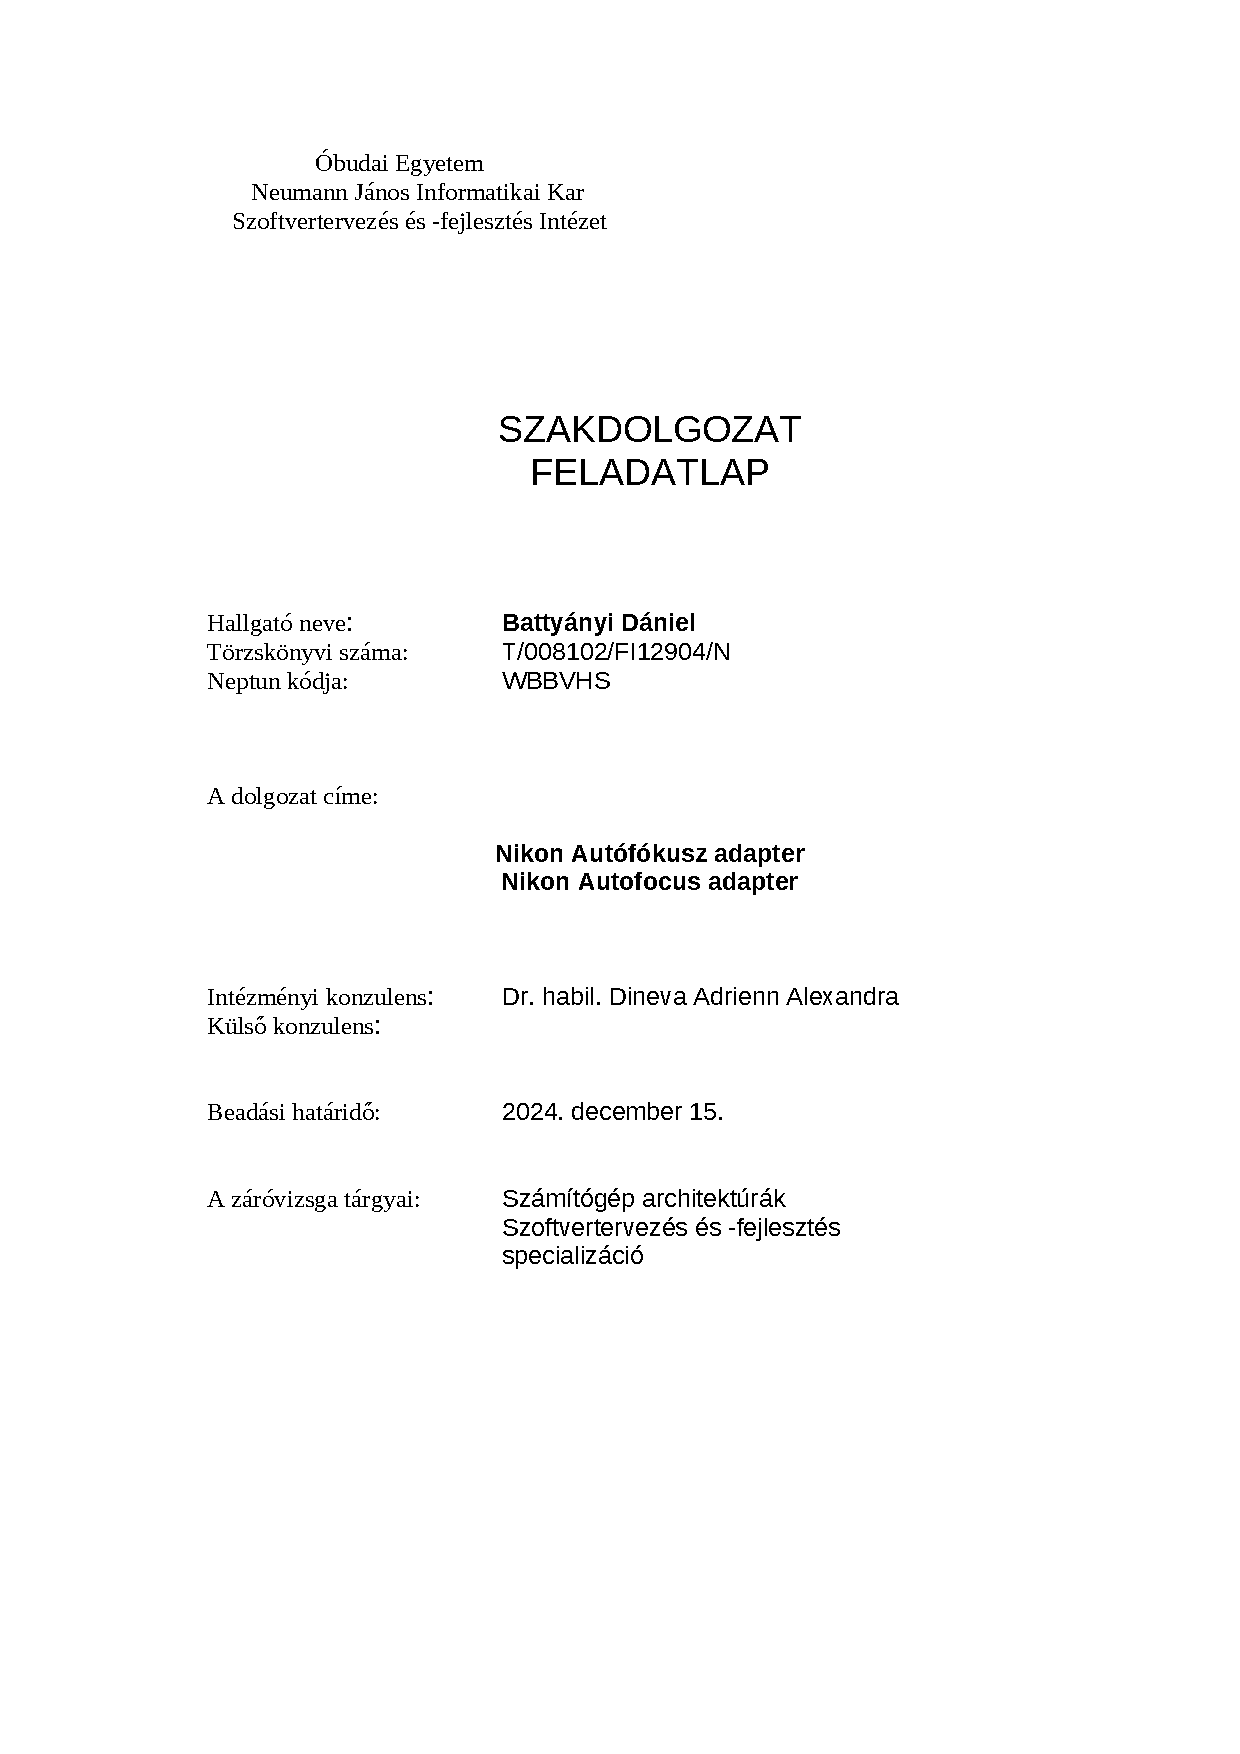
\includepdf[pages=-]{includes/feladatlap.pdf}
%
\includepdf[pages=-]{includes/nyilatkozat.pdf}
%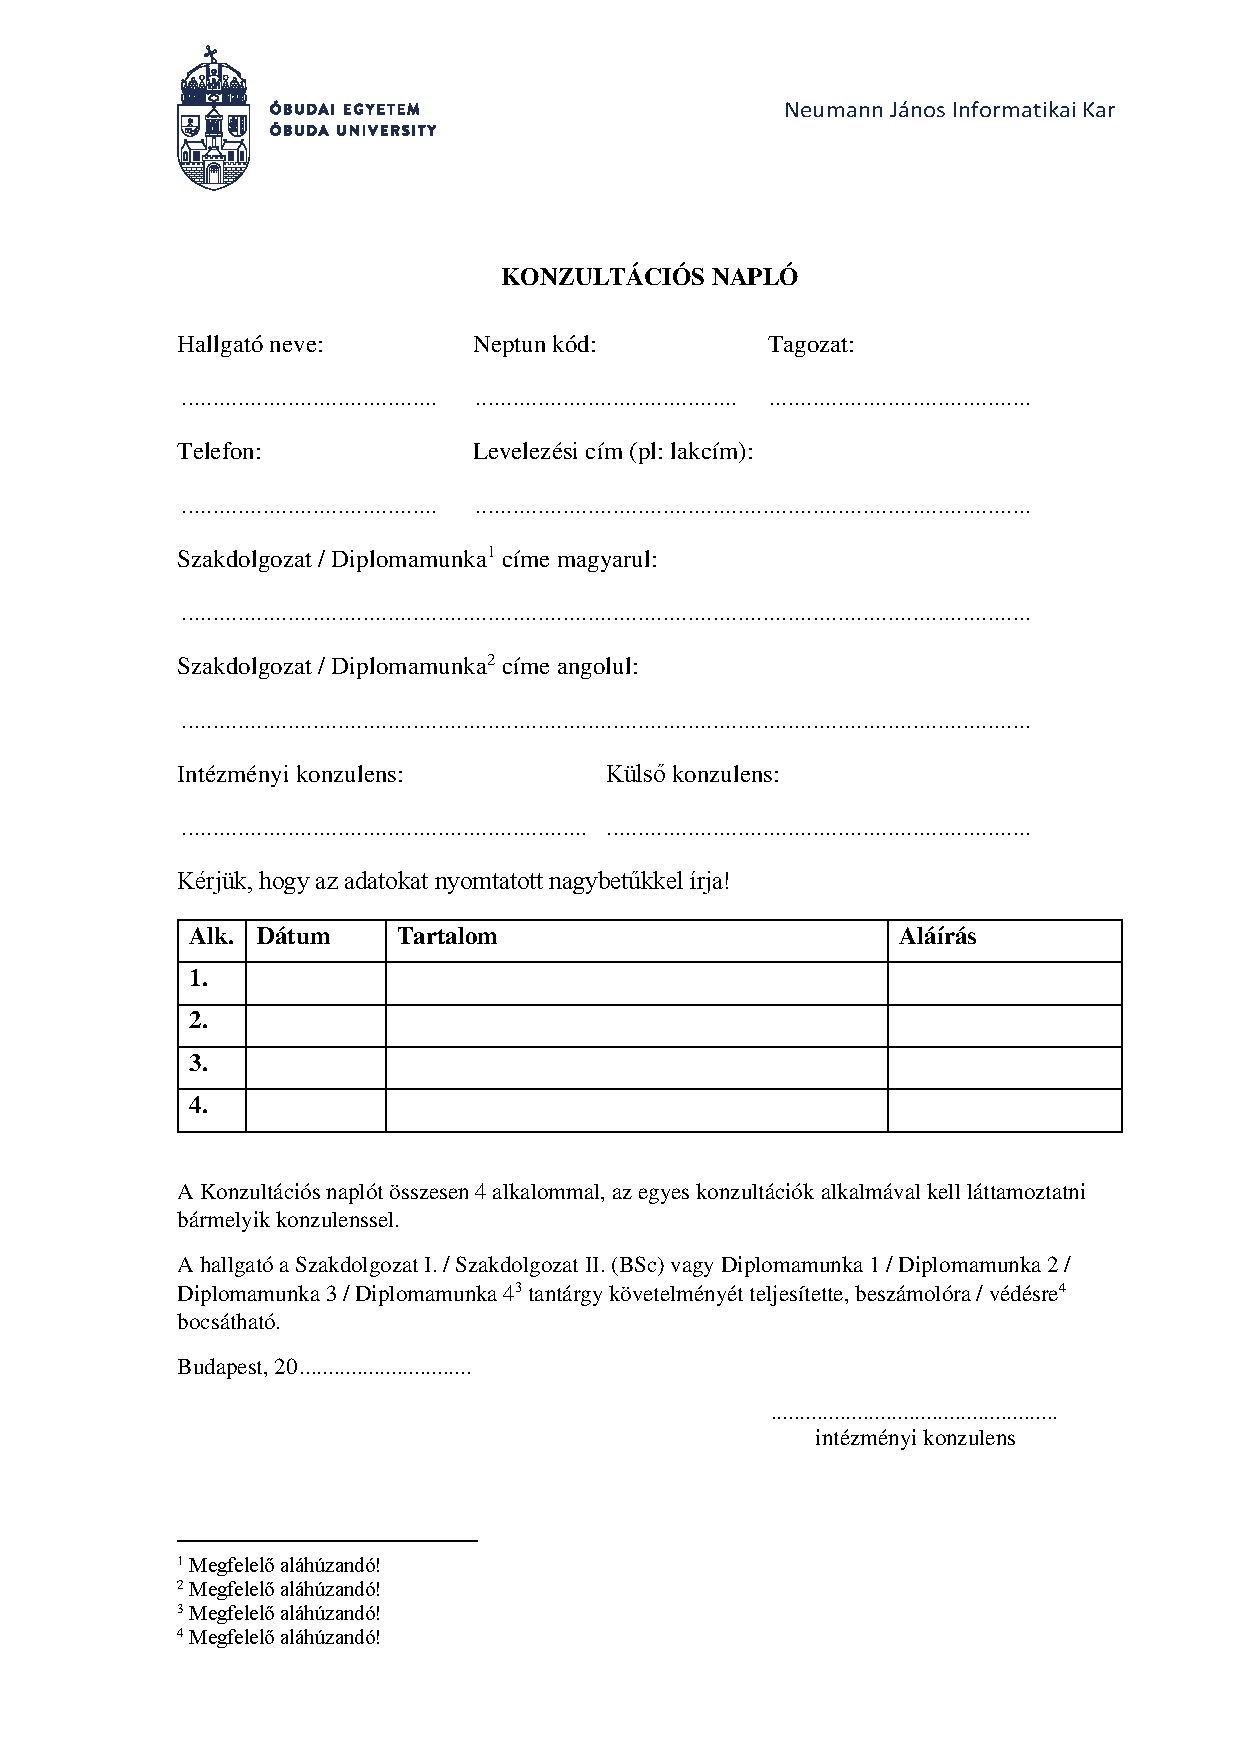
\includepdf[pages=-]{includes/konzultacios_naplo.pdf}


\newpage
\tableofcontents
\newpage

% csak a tartalomjegyzék után kezdődik a számozás
\pagenumbering{arabic}


% -----------------------------------------------------

% ITT KELL HOZZÁADNI A FEJEZETEKET, CÍM NAGYBETŰVEL:

\clearpage
\section{BEVEZETÉS}
\subsection{A projekt célja}
Egy olyan adaptert megalkotni, amely képes Nikon F-bajonettes objektíveket Nikon Z bajonettes fényképezőgépvázakra adaptálni, miközben azok megtartják teljes funkcionalitásukat. Bár hasonló adapterek léteznek, egyik sem képes visszaadni a régebbi AF és AF-D megjelölésű objektíveknek az automatikus fókuszáló képességét, amelyet beépített fókuszmotor hiányában a korábbi megoldások nem tartalmaznak. Ettől a hiányosságtól csökken a megtartható fényképek száma a fentebb említett lencsék esetén, ugyanis a fókusztávolságot manuálisan kell állítani, amely lassabb, és jóval nehezebb, mint a mutatás és fotózás (point and shoot). Ennek az új adapternek köszönhetően régebbi csúcsminőségű optikák is teljesen használhatóvá válnak, melyek között vannak olyan típusúak, amelyekből sosem készült új verzió.
\subsubsection{Az F-bajonett rövid története}
Az F-bajonettes objektívek története több mint 50 évre nyúlik vissza. A Nikon Corporation (eredeti nevén Nippon Kogaku K.K.) 1918 óta gyárt objektíveket és 1948 óta kamerákat. A vállalat 1959-ben bevezette a fényképezőgépéhez a Nikon F-hez az új F (immár) bajonettes csatlakozást\cite{Nikon_tori}, amellyel gyorsabban lehetett objektívet cserélni, valamint a csatlakozás is erősebb, precízebb lett. A Nikon tükörreflexes fényképezőgépei a mai napig ezt a bajonettet használják, legyenek azok digitálisak (DSLR) vagy analógok (SLR). A cég az autófókusz bevezetésekor hozott egy olyan döntést, aminek negatív következményét ez a projekt kívánja enyhíteni. Amíg a cég legfőbb riválisa a Canon ekkor új bajonettet vezetett be és a fókuszmotort az objektívbe helyezte el, ezzel szemben a Nikon megtartotta a csatlakozást, és csak módosította úgy, hogy egy csavarral a kameratestbe épített motor tudja állítani az optika fókuszát. Így bár az automatikus fókuszállítási sebesség (főleg a későbbiekben) csökkent, a korábbi autófókusz nélküli objektíveket is lehetett használni autófókuszos fényképezőgépvázakon és fordítva. Később azonban a Nikon vállalat is felismerte, az objektívekbe szerelt fókuszmotorok előnyeit, és a későbbi modellek már ilyen technológiákat használtak.
\subsubsection{A hivatalos Nikon FTZ adapter hiányosságai}
Amikor 2018-ban az új tükör nélküli fényképezőgépeket bemutatták\cite{Nikon_Z_Release}, akkor azok az új, Z bajonettjéhez készült hivatalos F bajonettes objektíveknek Z bajonettes vázra adaptáló adapterbe nem lett beépítve fókuszmotor, amelyekkel az idősebb AF és AF-D megjelölésű optikákat lehetne automatikusan fókuszálni, ami az alábbi táblázaton látható.

Bár könnyen meglehet, hogy ez egy jó pénzügyi döntés volt, hiszen ekkorra már a modern optikák közül egy sem támaszkodott a vázmotorra, de több professzionális fényképész is megkérdőjelezte a döntést. Ez többek között annak is köszönhető, hogy több népszerű és jó minőségű eszköz (pl.: Nikon Af 50mm 1.8(D), és a Nikon DC, (amely különleges, más fajta objektívek által nem nyújtott irányítást adott a kép fókuszon kívüli része felett) funkcionalitásából veszített az új platformon. A csalódottak között volt Ken Rockwell fotoblogger is, aki így fogalmazott: „A szomorú valóság az, hogy minél régebb óta fotózol Nikonnak, annál kevésbé szeretnéd az FTZ-t vagy az FTZ II-t, mert egyre kevésbé működnek az idősebb lencsékkel. (…) Nem tesz a Nikon nagy örökségének eleget.”\cite{Nikon_FTZ_Review}.
\clearpage
\section{KOMPATIBILITÁS}
\def\checkmark{\tikz\fill[scale=0.4](0,.25) -- (.25,0) -- (1,.7) -- (.25,.15) -- cycle;}

A bajonettcsatlakozók hosszas életútja miatt gyakran előfordul, hogy olyan új technológiák kerülnek beépítésre, amelyek nem kompatibilisek korábbi rendszerekkel. Ennek következtében meg kell határozni egy listát, amely tartalmazza a szükségesen kompatibilis eszközöket, és azok funkcionalitásait.

\subsection{Nikon F bajonettes objektívek és kiegészítők}

Az eredeti változat létrehozása óta rengeteg iteráción esett át a Nikon F bajonett, ezért kell választani egy referenciaverziót. Ez a dokumentum írásakor legújabb professzionális Nikon F bajonettes kamera, a Nikon D6-on is megtalálható vázbajonett. Ezen verziók következtében nem minden Nikon F bajonettes kamera kompatibilis minden más Nikon F bajonettes objektívvel, valamint nem minden funkció működik mindegyik párosítással. Ezért az alábbi kompatibilitási minimumok kerültek meghatározásra. 

\subsubsection{Inkompatibilis eszközök}

A különböző (elsősorban mechanikai) összeférhetetlenségek következtében az alábbi eszközök inkompatibilisek a referenciával, így az adapteren sem fognak szükségszerűen működni.
"
\begin{itemize}
	\item TC-16A AF telekonverterek
	\item Nem-AI objektívek (objektívek pre-AI expozíció csatlakozókkal)
	\item Objektívek, amik az AU-1 fókuszáló egységet igénylik (400mm f/4.5, 600mm f/5.6, 800mm f/8, 1200mm f/11)
    \item Fisheye (6mm f/5.6, 7.5mm f/5.6, 8mm f/8, OP 10mm f/5.6) halszemobjektívek
    \item 2.1cm f/4 objektív
    \item K2 toldógyűrűk
    \item 180–600mm f/8 ED objektívek (sorozatszámok: 174041–174180)
    \item 360–1200mm f/11 ED objektívek (sorozatszámok: 174031–174127)
    \item 200–600mm f/9.5 objektívek (sorozatszámok: 280001–300490)
    \item AF objektívek, amiket a F3AF fényképezőgépre készültek (AF 80mm f/2.8, AF 200mm f/3.5 ED, TC-16 AF telekonverterek)
    \item PC 28mm f/4 objektívek (sorozatszámok: 180900 or earlier)
    \item PC 35mm f/2.8 objektívek (sorozatszámok: 851001–906200)
    \item PC 35mm f/3.5 objektívek (régi típus)
    \item Reflex 1000mm f/6.3 objektívek (régi típus)
    \item Reflex 1000mm f/11 objektívek (sorozatszámok: 142361–143000)
    \item Reflex 2000mm f/11 objektívek (sorozatszámok: 200111–200310)
    \item IX-NIKKOR objektívek
\end{itemize}
"\cite{Nikon_D6_referencia_használati_utasítás}. 

\subsubsection{Kompatibilis eszközök funkciónalitása}

A kompatibilis objektíveknek az adapternek köszönhetően legalább az alábbi funkciónalitásokat kell elnyernijük a Z bajonettes fényképezőgépvázakon az adapternek köszönhetően:

\begin{itemize}
    \item "Manuális fókusz minden objektívvel."\cite{Nikon_D6_referencia_használati_utasítás}
    \item "VR a VR-el rendelkező objektíveken."\cite{Nikon_D6_referencia_használati_utasítás}
    \item "Pont fénymérés a CPU-val rendelkező objektíveken."\cite{Nikon_D6_referencia_használati_utasítás}
    \item "PC típusú objektíveknél a fénymérés és az automatikus expozícióbeállítás legalább "eltolás" és "döntés" nélkül működik."\cite{Nikon_D6_referencia_használati_utasítás}
    \item "A rekeszátmérő a rekeszátmérő gyűrű nélküli (G és E típusú) objektíveken a rekeszátmérőt az azt állító segéd parancstárcsával kell állítani."\cite{Nikon_D6_referencia_használati_utasítás_aperture}
    \item "A a rekeszátmérő gyűrűvel rendelkező objektíveken a rekeszátmérőt az objektíven található gyűrűvel kell állítani."\cite{Nikon_D6_referencia_használati_utasítás_aperture}
    
\end{itemize}

\clearpage

\begin{longtable}{|c|c|c|c|c|c|c|c|}
	%\centering
	%\begin{tabular}{|c|c|c|c|c|c|c|c|}
    	    \hline
    		\thead{Objektív vagy\\kiegészítő}  & \thead{Autófókusz}    & \multicolumn{2}{|c|}{\thead{Expozíciómód}}  & \multicolumn{3}{|c|}{\thead{Fénymérés}}   \\ 
            &  &  P, S & A, M & \makecell{Mátrix}& \makecell{Célpont,\\Középre-\\súlyozott} & \makecell{Csúcs-\\fényre\\súlyozott} \\ \hline
    		\makecell{G, E vagy \\D jelölésű\\AF-S AF-P\\és AF-I objektívek} & \checkmark    & \checkmark    & \checkmark  & \checkmark & \checkmark & \checkmark\\ \hline
            \makecell{PC Nikkor\\19mmf/4E ED} & \line(1,0){15} & \checkmark & \checkmark & \checkmark & \checkmark & \checkmark \\ \hline
            \makecell{PC-E Nikkor\\sorozat} & \line(1,0){15} & \checkmark & \checkmark & \checkmark & \checkmark & \checkmark \\ \hline
            \makecell{PC Micro 85mm\\f/2.8D} & \line(1,0){15} & \line(1,0){15} & M & \checkmark & \checkmark & \checkmark \\ \hline
            \makecell{AF-S/AF-I\\Telekonverterek} & \checkmark & \checkmark & \checkmark & \checkmark & \checkmark & \checkmark \\ \hline
            \makecell{Más AF Nikkor\\objektívek\\(Nikon F3AF\\kamerára készültek\\kivételével)} & \checkmark & \checkmark & \checkmark & \checkmark & \checkmark & \line(1,0){15} \\ \hline
            \makecell{AI-P Nikkor} & \line(1,0){15} & \checkmark & \checkmark & \checkmark & \checkmark & \line(1,0){15} \\ \hline
            \makecell{AI-,\\ AI-ra módosított\\és Nikon Series E \\objektívek} & \line(1,0){15} & \line(1,0){15} & \checkmark & \checkmark & \checkmark & \line(1,0){15} \\ \hline
            \makecell{Medical-NIKKOR\\120mm f/4} & \line(1,0){15} & \line(1,0){15} & \checkmark & \line(1,0){15} & \line(1,0){15} & \line(1,0){15} \\ \hline
            \makecell{Reflex-NIKKOR} & \line(1,0){15} & \line(1,0){15} & \checkmark & \line(1,0){15} & \checkmark & \line(1,0){15} \\ \hline
            \makecell{PC-NIKKOR} & \line(1,0){15} & \line(1,0){15} & \checkmark & \line(1,0){15} & \checkmark & \line(1,0){15} \\ \hline
            \makecell{AI-típusú\\Telekonverter} & \line(1,0){15} & \line(1,0){15} & \checkmark & \checkmark & \checkmark & \line(1,0){15} \\ \hline
            \makecell{PB-6\\csatlakoztatható\\fókuszcsúszka} & \line(1,0){15} & \line(1,0){15} & \checkmark & \line(1,0){15}& \checkmark & \line(1,0){15} \\ \hline
            \makecell{Auto toldógyűrűk\\(PK-series 11A,\\ 12 vagy 13;\\ PN-11)} & \line(1,0){15} & \line(1,0){15} & \checkmark & \line(1,0){15}& \checkmark & \line(1,0){15} \\ \hline 
    %\end{tabular}
	\caption{Nikon F bajonettes objektívek szükséges funkcionalitása \cite{Nikon_D6_referencia_használati_utasítás}}
	\label{tab:ur5}
\end{longtable}

\subsection{Nikon Z bajonettes fényképezőgépvázak}

Mivel Nikon Z bajonettes fényképezőgépek csak 2018 ősze\cite{Nikon_Z_Release} óta kaphatók, ezért bár a kihozott kamerák között helyenként nagy funkcionalitásbeli különbség van, a csatlakozó még nem esett át változtatásokon. Emmiatt a dokumentum írásakor elérhető összes Nikon Z bajonettcsatlakozással rendelkező fényképezőgéppel használhatónak kell lennie az adapternek, és azokon ugyan azokat a funkcionalitásokat kell biztosítania.
\clearpage
\section{NIKON F BAJONETT}
%A Nikon F bajonett a modern SLR és DSLR fényképezőgépek által használt objektívcsatlakozás, amely tartalmaz mechanikus elemeket, valamint tartalmazhat elektronikus csatlakozásokat is.

"Nikon SLR-eken és NIKKOR objektíveken, a Nikon F 1959-es bemutatásától a mai modellekig használatos bajonett típusú F-csatlakozás egy kommunikációs kapcsolat Nikon SLR-ek és Nikon objektívek között.

Erős felépítéséről és kiemelkedő megbízhatóságáról emlékezetessé vált, az F-Csatlakozás kiemelkedő a NIKKOR objektívekkel való magasfokú kompatibilitásnak és egy olyan dizájnnak köszönhetően, amely képes magába foglalni későbbi fejlődéseket. A Nikon fenntartotta a csatlakozás alap struktúráját az 50 éven át tartó használata során, és jelenleg nagyjából 400 különböző objektív kompatibilis a rendszerrel. A Nikon F-Csatlakozás egyik legnagyobb előnye, hogy lehet egy nagy objektívkollekcióból választani, amibe beletartoznak az AF NIKKOR, AF-S (Silent Wave Motor) és PC-E perspective-control (perspektíva kontroll) NIKKOR objektívek is.

Az F-Csatlakozás és a NIKKOR objektívek képességeinek adaptálásával és bővítésével, Nikon beépített technológiákat, mint például autófókusz, fejlett fénymérés, távolság információ technológia, elektronikus rekeszátmérő irányítás a G-típusú NIKKOR-ban, VR (Vibráció Redukció) képstabilizálás és Silent Wave Motor (AF-S), ezáltal fenntartva egy jelentős fokú kompatibilitást, ezzel demonstrálva egy folyamatos elköteleződést o fényképészek iránt."\cite{Nikon_F_mount-ról}

%Used on Nikon SLRs and NIKKOR lenses from the introduction of the Nikon F in 1959 to current models, the bayonet-type F-Mount is the communication link between Nikon SLRs and NIKKOR lenses.

%"Noted for its rugged construction and outstanding reliability, the F-Mount is distinctive also for its degree of compatibility with NIKKOR lenses and a design that can accommodate future system advances. Nikon has maintained the basic structure of the mount for the 50 years of its use, and currently some 400 different NIKKOR lenses are compatible with the system.
%One of the biggest advantages of the Nikon F-Mount is that you're able to choose from a large selection of lenses including: AF NIKKOR and AF-S (Silent Wave Motor) and PC-E perspective-control NIKKOR lenses.

%By adapting and extending the capability of the F-Mount and NIKKOR lenses, Nikon has incorporated technologies like autofocus, advanced metering, distance information technology, electronic aperture control in G-Type NIKKOR, VR (Vibration Reduction) image stabilization and Silent Wave Motor (AF-S) technology, thus maintaining a significant degree of compatibility and demonstrating an ongoing commitment to photographers."

\paragraph{Felépítése}

%IDE KELL EGY RÖID ISMERTETÉS A CSATLAKOZÁS RÖGZÍTÉSÉRŐL
"(...) egy F-csatlakozás nem egy menetes csatlakozás; hanem, egy bajonett csatlakozás. A bajonett csatlakozások nagyon jók fényképezéshez, mivel álataluk a kamera felhasználója könnyeb és hatékonyan tud objektíveket különböző körülményekhez cserélni, és könnyen integrálhatóvá teszik az elektronikus funkciókat (írisz/fókusz irányítás), mivel ezek kiszémítható, pontos mechanizmusok."\cite{Nikon-bajonett}
%an F-mount is not a threaded mount; rather, it is a bayonet
%mount. Bayonet mounts are great
%for photography, as they allow the
%user of the camera to swap lenses
%out quickly and efficiently for different scenarios, and allows for the
%easy integration of electronic features (iris/focus control) since they
%are a clocked mechanism.

%Ez itt a \ref{fig:AF_kontakt} ábra.
\begin{figure}[H]
	\centering
	\includegraphics[width=0.5\linewidth]{img/Nikon_50mm_1.8_kontaktok.jpg}
	\caption{Elektronikus kontaktok Nikon AF típusú objektíven}
	\label{fig:AF_kontakt}
\end{figure}

\begin{figure}[H]
	\centering
	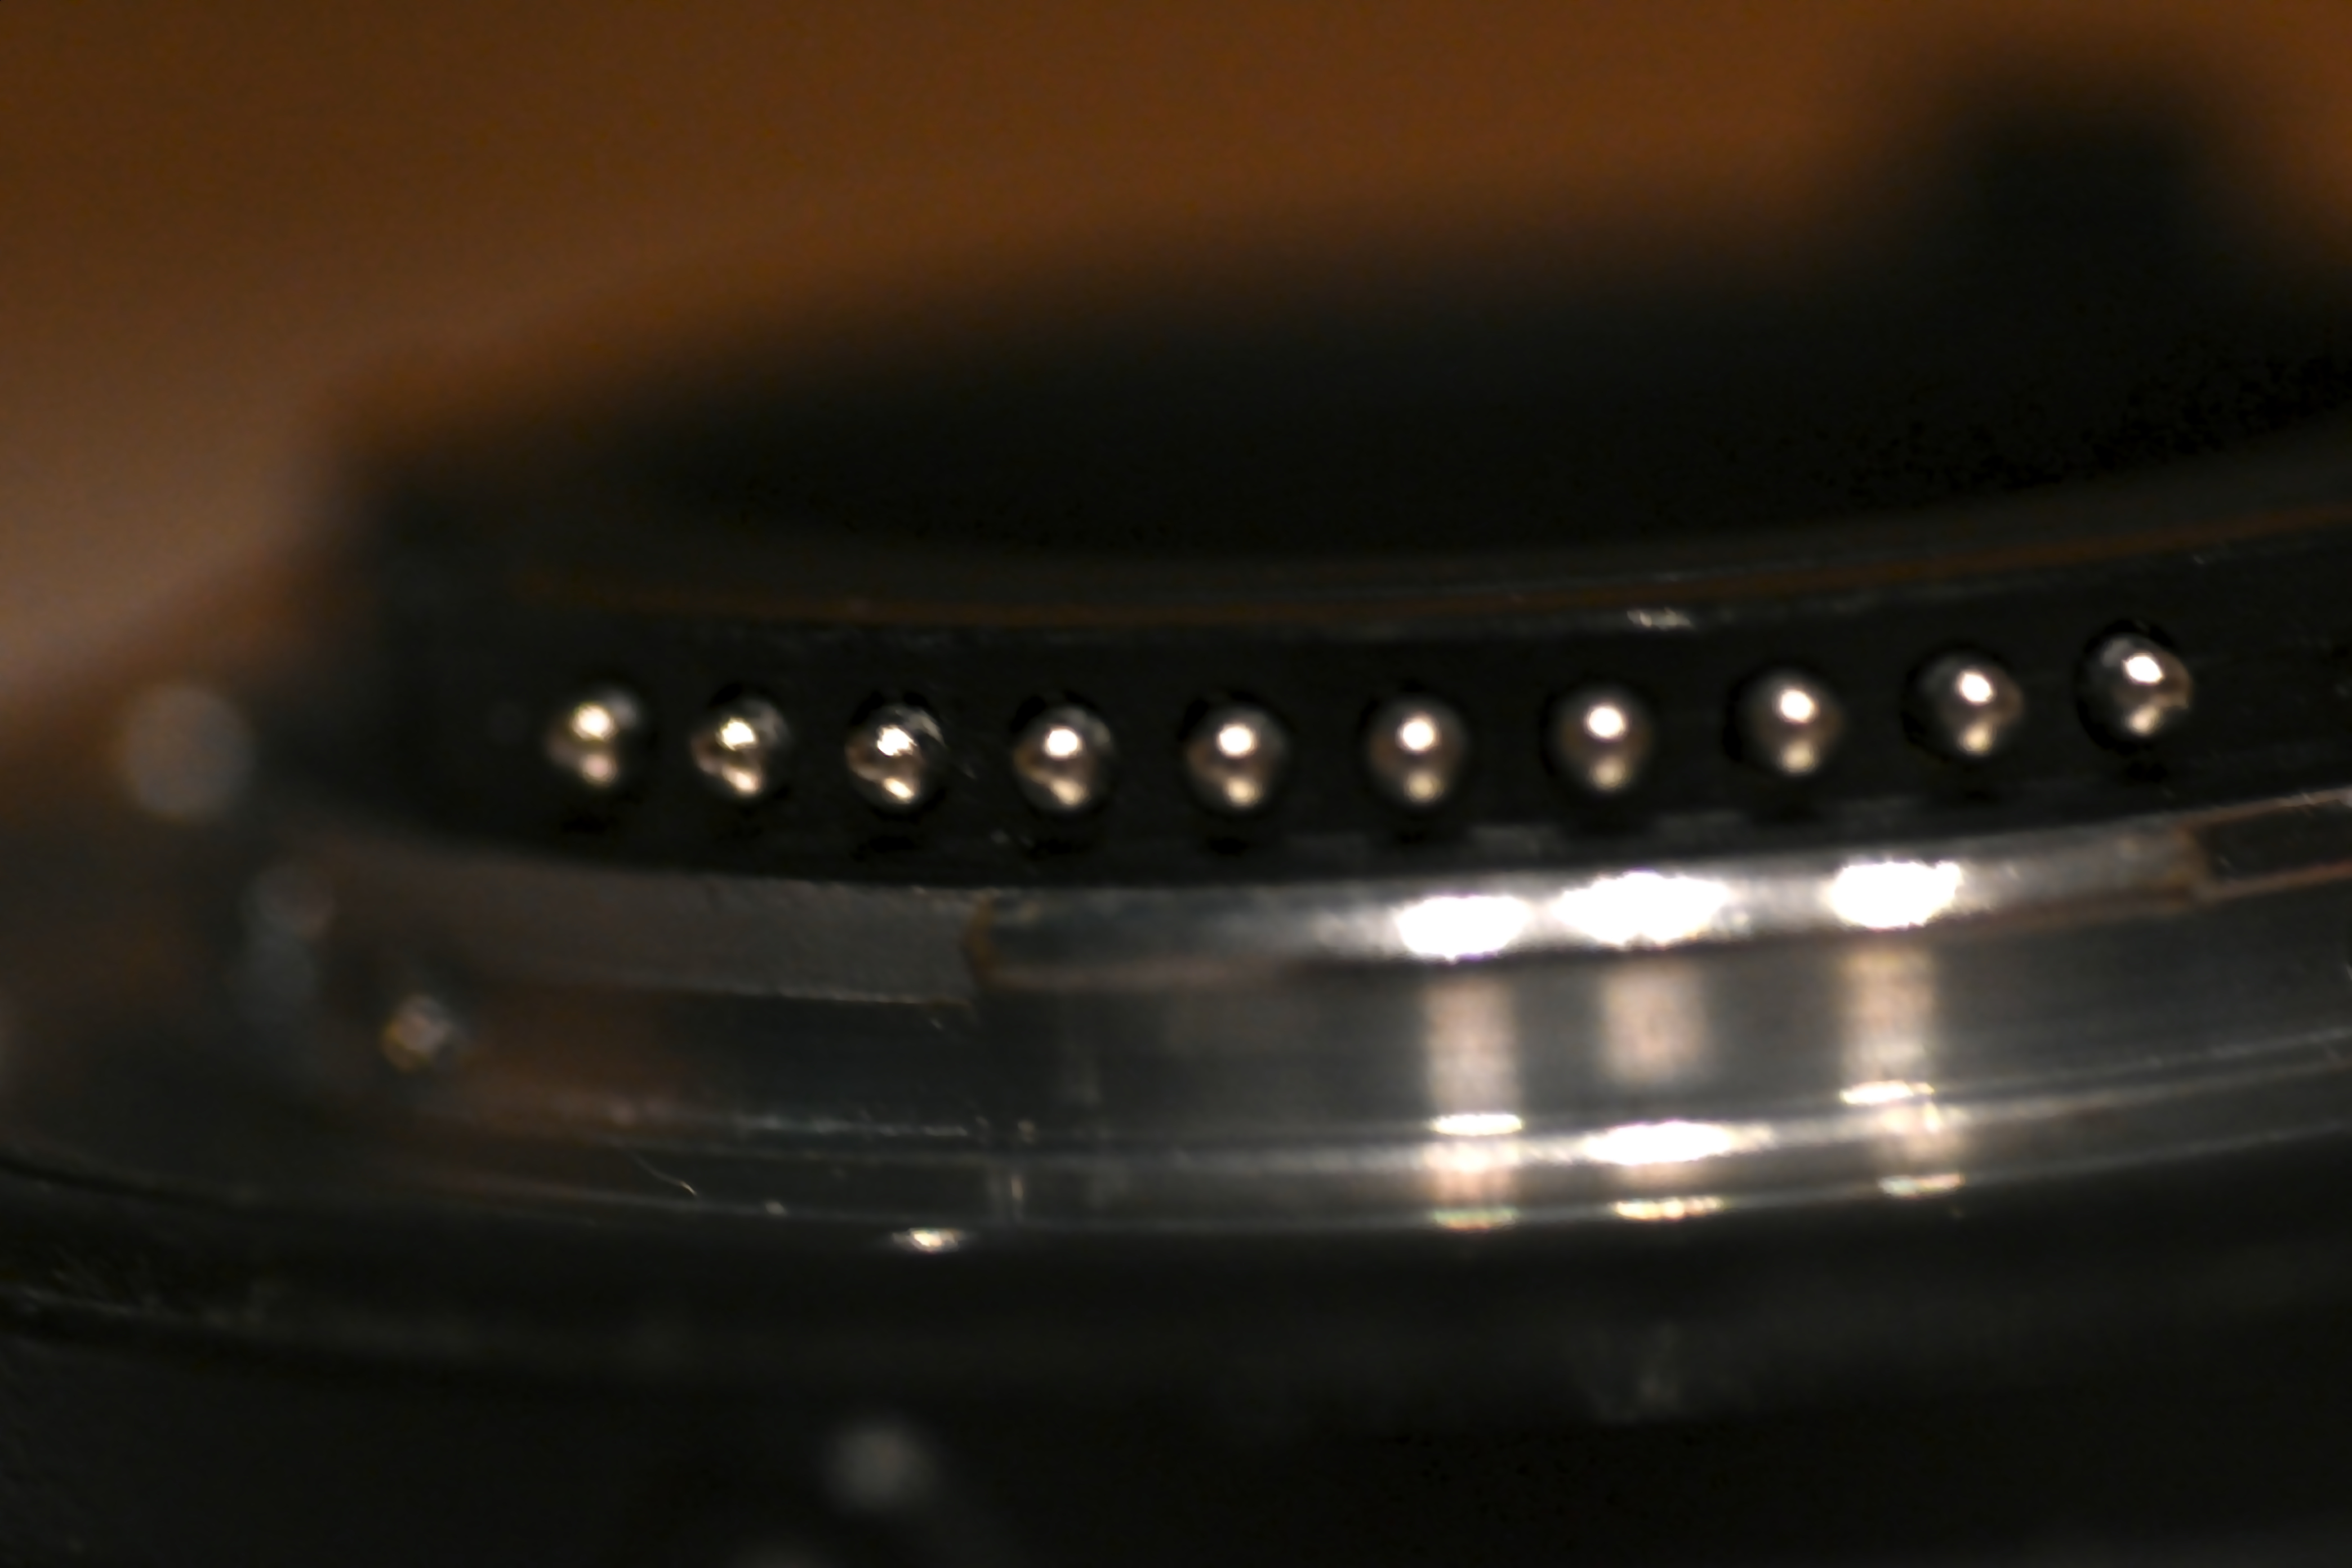
\includegraphics[width=0.5\linewidth]{img/Nikon_17-55_kontaktok.jpg}
	\caption{Elektronikus kontaktok Nikon AF-S DX 17-55mm f/2.8 G objektíven}
	\label{fig:G_kontakt}
\end{figure}

% \begin{figure}[H]
% 	\centering
% 	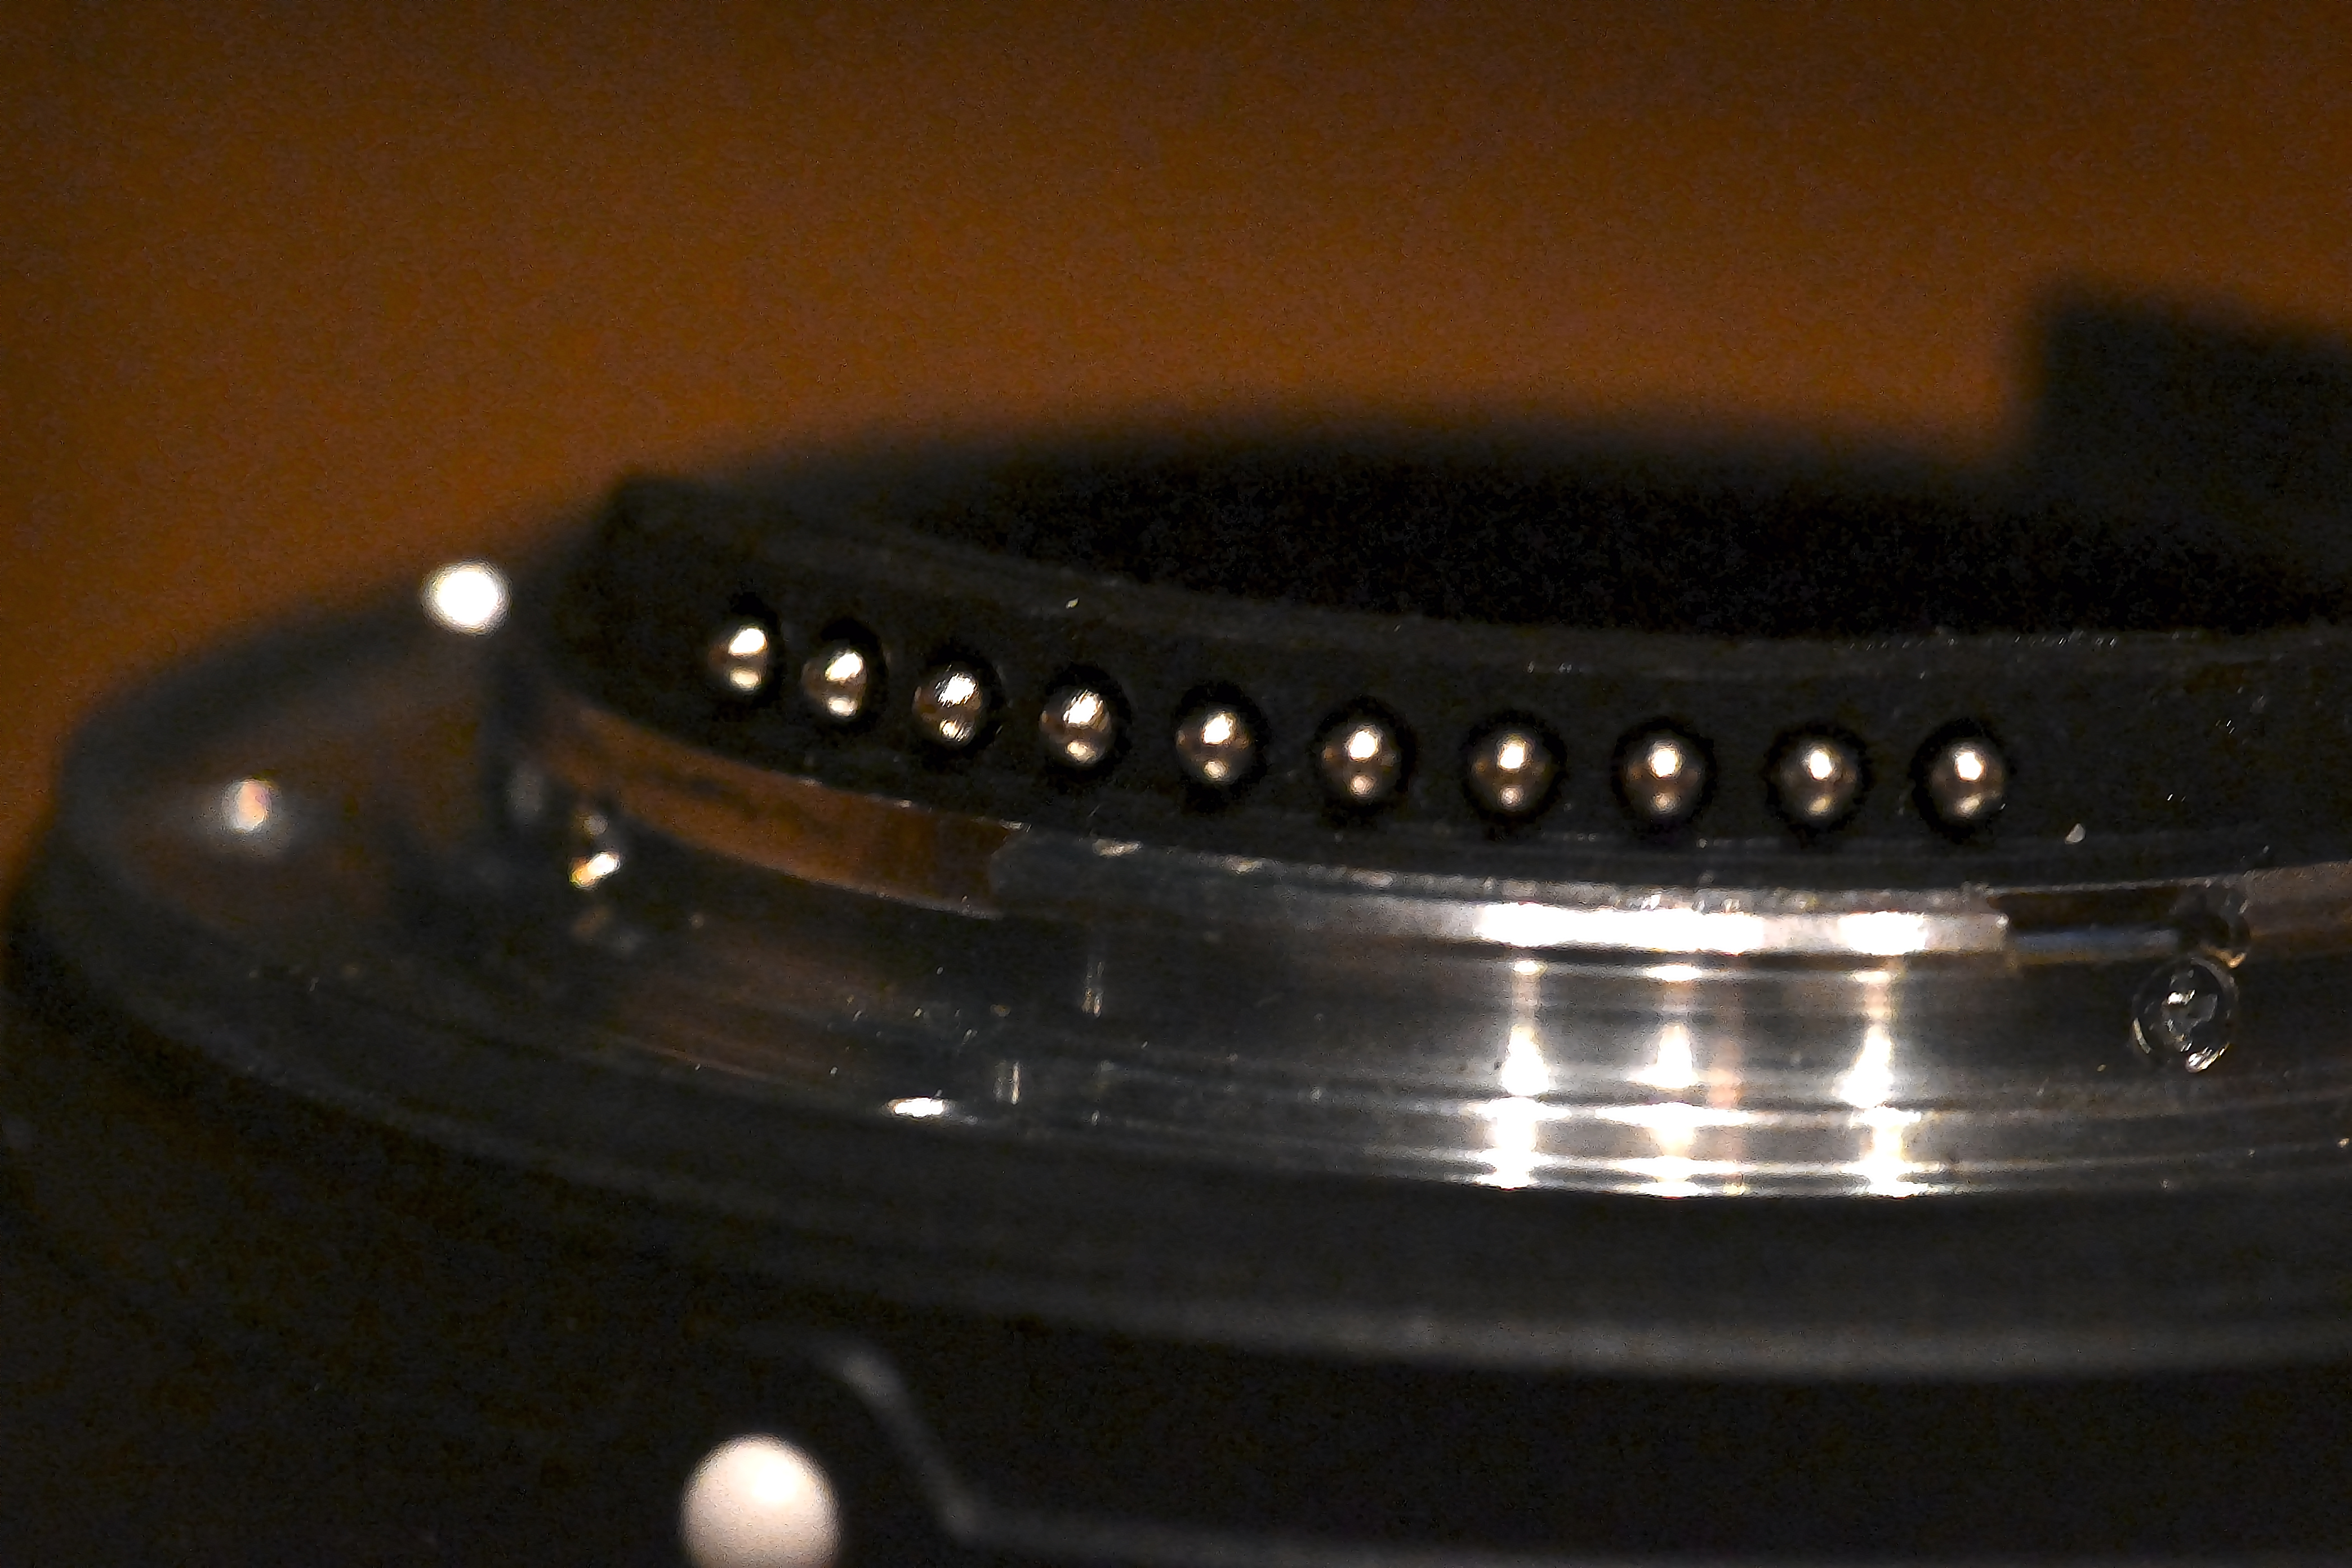
\includegraphics[width=0.5\linewidth]{img/Nikon_70-200E_kontaktok.jpg}
% 	\caption{Elektronikus kontaktok Nikon AF-S 70-200mm E FL ED VR objektíven}
% 	\label{fig:E_kontakt}
% \end{figure}
\subsection{Rögzítés}
A csatlakozás felettébb tartós\cite{Nikon_F_mount-ról}.
Az objektívet az azon és a fényképezővázon feltüntetett jelzések mentén kell a váz csatlakozójára illeszteni, majd elforgatni.
A megfelelő illesztés során az objektív csatlakozója enyhén belecsúszik a vázoldali részbe, ahol a kettő gyűrűjének a kialakítása vezeti az objektívet a forgatás során.
A túl, vagy rossz irányú forgatást ütközők akadályozzák meg.
Amikor az objektív a megfelelő pozícióba ér, egy rugó által kitolt tüske rögzíti azt.
Levételkor egy gomb elnyomásának, vagy egy rugós kapcsoló elhúzásának köszönhetően ez a tüske visszahúzódik, így engedélyezve az objektív levehető pozíció felé mozgatását.

\subsection{Rekeszátmérő állítás}
A fényképezés során legtöbb esetben a fókuszálást nem a kiválasztott rekeszértékkel végzi a kamera (automatikusan) vagy a fényképész (manuálisan).
Emiatt a rekeszértéket a fénykép készítése előtt a megfelelő értékre kell állítani.
Ez régebbi objektíveknél manuálisan történt (ezek nem használhatóak a modern SLR és DSLR rendszerekkel), de az F bajonettes objektíveknél ez már autómatikusan az "autómatikus diafragmánaknak" köszönhetően valósul meg.
Ilyenkor amennyiben a rekeszátmérő nem esik egy előre meghatározott érték alá, a fókuszáláskor használatos rekeszátmérő megegyezik a kép készítésekor felvett rekeszátmérővel. Ellenkező esetben a fénykép készítésekor a diafragma a nyilt (\ref{fig:17-55_nyilt} ábra) állásáról a zárt (\ref{fig:17-55_zart} ábra) állására ugrik át, ami már a beállított érték.
Ennek a folyamatnak minél gyorsabbnak kell lennie, hogy a fényképen az látszódjon, amit a kezelő a gomb lenyomásakor beállított. \cite{Practical_design_considerations_for_modern_photographic_optics}
\paragraph{Kívánt érték megadása}
A kívánatos érték érték a Nikon rendszereken kettő féle képpen történhet meg:
\begin{itemize}
    \item Objektíven a rekeszátmérő gyűrű segítségével.(G és E objektíveken nem elérhető)
    \item A kamerán található rekeszátmérő állító kerékkel.
\end{itemize}
Amennyiben az objektív mindkét lehetőséget használatát megengedi, a vázon a fényképésznek be kell állítania, hogy melyik módszert szándékozik használni.
Ha a felhasználó a fényképezőgépen akarja állítani az értéket, egy rekeszátmérő gyűrűvel rendelkező objektív használatánál, a rekeszátmérőt az objektíven található gyűrűn a legnagyobb f-értékre kell állítania a felhasználónak.
Erre a lépésre fényképezőgép is figyelmeztet.\cite{Nikon_D6_referencia_használati_utasítás}

\subsection{Elektronikus csatlakozás}
% UPDATE WITH NIKON HACKERS STUFF. REFERENCE REPAIR MANUALS FOR THE CONTACTS.
Az összes CPU-val rendelkező objektív csatlakozásán találhatóak elektronikus kontaktok.\cite{Nikon_CPU}
Ezek feladata az, hogy gyors kommunikációt létesítsenek az objektív és a kameraváz között.

Ezeken kívül a kamera elelektromos árammal is ellátja ezeket az eszközöket, ezzel biztosítva azt, hogy az objektívek és kiegészítők megfelelően, külső áramforrás nélkül tudjanak üzemelni.
AF-I, AF-S és AF-P esetében az objektívbe beépített fókuszmotornak is ez szolgál áramforrásként.

A CPU kontaktok száma objektívek között váltózó.\cite{Nikon_CPU}
A referencia kameraváz, valamint a hivatalos Nikon FTZ adapter is 8 tűvel rendelkezik, így ez az adapter is ennyit fog használni.
Ennél több nem kamera vázakon, csak objektíveken és telekonvertereken, ezért vázszimulációhoz szükségtelen.

\begin{figure}[H]
	\centering
	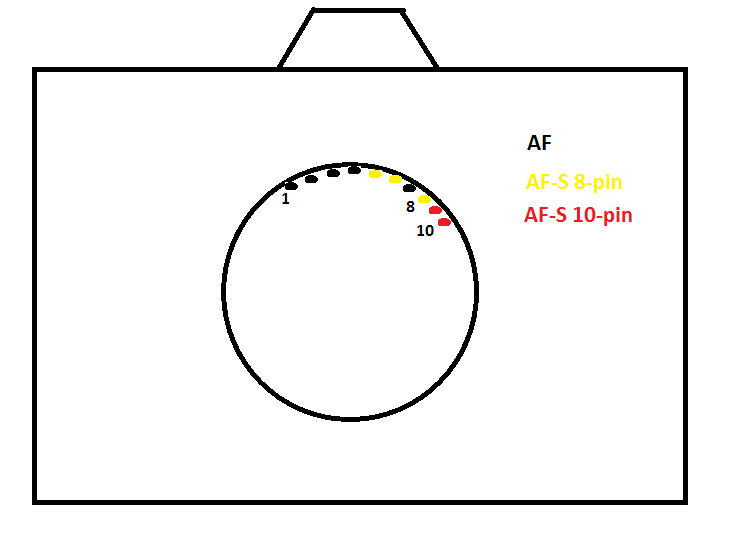
\includegraphics[width=0.5\linewidth]{img/Fmount.png}
	\caption{Nikon fényképezőgépvázon található elektromos kontaktok}
	\label{fig:FMount}
\end{figure}
\keepXColumns
\begin{tabularx}{\textwidth}{|c|c|c|c|X|}
    \hline
    \rowcolor{lightgray}\textbf{Tű} & \textbf{AF} & \textbf{AF-S 8-tűs} & \textbf{AF-S 10 tűs} & \textbf{Leírás} \\
    \hline
    \endfirsthead
    
    \hline
    \rowcolor{lightgray}\textbf{Tű} & \textbf{AF} & \textbf{AF-S 8-tűs} & \textbf{AF-S 10 tűs} & \textbf{Leírás} \\
    \hline
    \endhead
    
    1/A & x & x & x & 5V Vcc táp \\
    \hline
    2/B & x & x & x & Soros RW kiválasztó / \textit{kézfogás} \\
    \hline
    3/C & x & x & x & Soros órajel \\
    \hline
    4/D & x & x & x & Soros adat IO \\
    \hline
    5/E &   & x & x & Impulzussor. Pulzusok száma: fókuszváltás mennyisége. Pulzusok frekvenciája: fókuszváltás sebessége. M/A (Manual autofocus override) módban aktív, M (Manual) módban inaktív. Kamerával közli a fókusz változását. Nyílt kollektor kimenet. Kamerának logikai magas állapotba kell raknia a működéshez. 0xEA parancs 1 bitje irányítja a kimenetét. \\
    \hline
    6/F &   & x & x & Vmotor táp Zoom, VR, Autofókusz számára. ~6.2V (D800, D5100, F5) \\
    \hline
    7/G & x & x & x & Föld \\
    \hline
    8/H &   & x & x & Pin 5 90° fáziseltolásban. Az eltolás iránya jelzi a fókusz irányát. Csak Pro kamerákon (opcionális). 0xEA parancs 0 bitje irányítja. \\
    \hline
    9/I &   &   & x & Telekonverter indikátor/kommunikáció. \\
    \hline
    10/J &   &   & x & Telekonverter indikátor/kommunikáció. \\
    \hline
    \caption{Nikon F csatlakozás kontaktok szerepei.}
    \label{tab:nikon_pins}
\end{tabularx}

\subsection{Kommunikáció}
A Nikon F bajonettcsatlakozónál az objektív és a fényképezőgépváz közötti kommunikáció történhet mechanikai(AI, AI-S jelölésű objektívek)\cite{Lens_naming}, elektronikai (E jelölésű objektívek)\cite{Lens_naming}, valamint egyszerre mechanikai és elektronikai (AI-P, AF, AF-I, D és G jelölésű objektívek)%\cite{Nikon_naming_convention}
\cite{Nikon_CPU}úton. Ezeken a kategóriákon belüli csatlakozók között lehetnek további különbségek az eszközök funkcióitól függően.

\subsubsection{Elektronikus adatkommunikáció:}
A kamera által az objektívvel elektronikusan közölt információk közé tartoznak:
\begin{itemize}
    \item Amennyiben az objektív nem AF típusú autófókuszmechanizmust tartalmaz, a fókuszáláshoz szükséges adatok.
    \item E jelölésű objektíveknél rekeszátmérőt állító jelek.
\end{itemize}
Az objektív által a kamerával elektronikusan közölt információk közé tartoznak:
\begin{itemize}
    \item Az objektívet vagy kiegészítőt azonosító információ.
    \begin{itemize}
        \item Az objektív maximális rekeszátmérője.
        \item Az objektív minimális rekeszátmérője.
        \item Az objektív elnevezése.
        \item Az objektív gyújtótávolsága.%\cite{Nikon_naming_convention}
    \end{itemize}
    \item Az objektív jelenlegi rekeszátmérője.
    \item Az objektív autófókuszálásához szükséges információk.
    \item D, G és E jelölésű objektíveknél az objektíven beállított fókusztávolság.
    \item Egyéb fénymérést segítő információ.
\end{itemize}

Ennek pontos működése nem ismert, hivatalos Nikon dokumentáció nem érhető el, viszont online közösségek által végzett kutatások alapján nem hivatalos, részleges specifikációk elérhetőek.
\paragraph{Adatátvitel}
SPI-szerű soros, szinkron, kommunikációs protokollal történik, amely a követlezőekben tér el a szabványtól:
\begin{itemize}
    \item PS (periféria kiválasztó) el van hagyva.
    \item PI (periféria bemenet) és (PO - periféria kimenet) ugyan azon az adatúton helyezkedik el
    \item Kézfogásvonal került hozzáadásra.
\end{itemize}

A protokoll 3-as módban üzemel:
\begin{table}[H]
    \centering
    \begin{tabular}{|c|c|c|c|c|}
        \hline
        \rowcolor{lightgray} SPI mode & Polaritás regiszter & Fázis regiszter & Küldő Óra ág & Beolvasó óra ág \\
        \hline
        3 & logikai magas & logikai magas & zuhanó ágon & emelkedő ágon \\
        \hline
    \end{tabular}
\end{table} \textbf{Polaritás:} Óra adatküldésen kívöli állapota.\\
\textbf{Fázis:} Az óra melyik ágán történik a mintavétel, bitküldés.

Az adat bájtonkként kerül továbbításra a legkisebb helyiértékű bittel kezdve.
Az alapértelmezett órajel 96~kHz, azonban újabb AF-S objektívek esetében ez akár 156~kHz-re is növekedhet (pl. a \texttt{0x40} parancs után).
Az adapternek is célszerű ezt az órajelet használnia az alacsonyabb reakcióidő érdekében.

\paragraph{Kommunikációs szekvencia}

A kommunikációt mindig a fényképezőgép váza kezdeményezi azáltal, hogy 
a \textit{kézfogás} vonalat alacsony szintre húzza 1600~$\mu$s ideig 
(96~kHz-en), vagy 100~$\mu$s-ig (156~kHz esetén), majd elengedi. 

Ezután az objektív húzza le a \textit{kézfogás} vonalat, jelezve, hogy készen 
áll a parancs fogadására. Ha az objektív nem válaszol időben, a parancs 
megszakad.

Egy parancs egyetlen bájtból áll, de azt további adatbájtok követhetik, 
amelyek iránya és száma az eszközök által előre ismert, konstans.
Az adatátvitelt bármelyik fél megszakíthatja: az objektív nem húzza le újra a \textit{kézfogás} vonalat, vagy a váz nem ad órajelet. 

Ha körülbelül 5ms-ig nincs adatforgalom, a kommunikációs ciklus megszakítottnak tekintendő.

Fontos: a modern objektívek nem küldenek vissza \texttt{0xFF} bájtot 
ismeretlen parancs esetén. Ehelyett egyszerűen megszakad a kommunikáció.

\paragraph{Ismert parancsok}

\begin{longtable}{|c|p{3.5cm}|p{3.5cm}|p{5cm}|}
    \hline
    \rowcolor{lightgray}
    \textbf{Parancs} & 
    \textbf{Paraméterek (váz $\rightarrow$ obj.)} & 
    \textbf{Válasz (obj. $\rightarrow$ váz)} & 
    \textbf{Leírás} \\
    \hline
    \endfirsthead
    
    \hline
    \rowcolor{lightgray}
    \textbf{Parancs} & 
    \textbf{Paraméterek (váz $\rightarrow$ obj.)} & 
    \textbf{Válasz (obj. $\rightarrow$ váz)} & 
    \textbf{Leírás} \\
    \hline
    \endhead
    
    \hline
    \multicolumn{4}{r}{\textit{Folytatás a következő oldalon}} \\
    \endfoot
    
    \endlastfoot
    
    \texttt{0x26} & – & 8 bájt & Ismeretlen funkció (feltételezhetően olvasási kísérlet) \\
    \hline \texttt{0x27} & – & 40 bájt & Objektív státusz-lekérdezés (workaround Rokinon bug miatt) \\
    \hline\texttt{0x28} & – & 44 bájt & Objektív státusz és ID információ lekérése \\
    \hline \texttt{0x40} & \texttt{00 00 01 04 00 00 01} & \texttt{02 1A} (D5100), \newline \texttt{02 1B} (D800) & Objektív képességeinek lekérdezése, sebességváltás 156~kHz-re \\
    \hline \texttt{0x41} & \texttt{02 1A} & – & A korábban küldött adatok visszaolvasása \\
    \hline \texttt{0xC2} & – & 4 bájt & Ismeretlen funkció \\
    \hline \texttt{0xC5} & – & 8 bájt & Ismeretlen funkció \\
    \hline \texttt{0xD1} & – & 1 bájt & VR bekapcsolása (funkció bájt ismeretlen) \\
    \hline \texttt{0xD2} & – & 3 bájt & VR bekapcsolása (funkció bájtok ismeretlenek) \\
    \hline \texttt{0xD3} & – & 1 bájt & Csak VR objektíveken, VR állapottól függetlenül \\
    \hline \texttt{0xD4} & – & 1 bájt & Csak VR objektíveken, VR állapottól függetlenül \\
    \hline \texttt{0xD5} & – & 4 bájt & Csak VR objektíveken, VR állapottól függetlenül \\
    \hline \texttt{0xE0} & – & 4 bájt & AF adott távolságra és irányba \newline (2–3. bájt: 15 bites little-endian, előjeles) \\
    \hline \texttt{0xE3} & – & – & AF motor leállítása \\
    \hline \texttt{0xE7} & – & 1 bájt & Ismeretlen funkció \\
    \hline \texttt{0xE8} & – & 5 bájt & Gyors AF pozícióra, majd folyamatos sebesség \\
    \hline \texttt{0xEA} & – & 1 bájt & GMR visszajelzés vezérlése (bit0,1: lábak 8,5) \\
    \hline \texttt{0xEC} & – & 3 bájt & AF adott irányba és sebességgel \newline (bájt0: bit3 végállás/fordulás, bit4 irány; \newline bájt1–2: sebesség m, n paraméterek) \\
    \hline \caption{Jellemző objektív parancsok és kiegészítések. \cite{nikonhacker_fmount}, \cite{lainy_nikonlens_issue1}}
\end{longtable}

Bizonyos nem gyári objektívek (pl. RokiBowYang 8~mm f/3.5) \texttt{0xFF} 
válasszal reagálnak ismeretlen parancsokra, de ezt modern vázak (pl. D5100, 
D800) figyelmen kívül hagyják.\cite{nikonhacker_fmount}, \cite{lainy_nikonlens_issue1}


\subsubsection{Elektronikus autómatikus diafragma}
Az E és csakis az E jelölésű objektívek a soros interfésszel állítják be a rekeszátmérőt.
"Egy elektromágneses diafragma mechanizmus van beépítve ezen objektívek testébe, amit elektromos jelek irányítanak a fényképezővázból. "\cite{Lens_naming}

\subsection{Mechanikus kommunikáció}
A CPU-val nem rendelkező objektívek nem tudnak elektronikus úton kommunikálni, ezért a kommunikáció jelentős mértékben lekorlátozódik, és csak kevés információ, lassú cseréje lehetséges.
Ennek ellenére a visszafelé kompatibilitás megőrzése érdekében és a technológia egyszerűségének köszönhetően, az E jelölésű objektíveken kívűl minden objektív rendelkezik ilyen kapcsolatokkal.
A fényképezőváz által az objektíveken mechanikusan állított értékek:
\begin{itemize}
    \item AF objektívek esetén fókusztávolság. (\ref{fig:AF_csavar}-es ábra)
    \begin{figure}[H]
    	\centering
    	\includegraphics[width=0.5\linewidth]{img/Nikon_50mm_1.8_AF_csavar.jpg}
    	\caption{Fókuszállító csavar Nikon AF típusú objektíven}
    	\label{fig:AF_csavar}
    \end{figure}
    \item Rekeszátmérő (Az E jelölésű objektívek kivételével).
    \begin{itemize}
        \item Nyílt vagy zárt pozíció \ref{fig:G_rekeszkar}
        \begin{figure}[H]
        	\centering
        	\includegraphics[width=0.5\linewidth]{img/Nikon_17-55_rekeszkar.jpg}
        	\caption{Mechanikus kar a rekesz nyitására és zárására használt álláskapcsoló G típusú Nikon objektíven}
        	\label{fig:G_rekeszkar}
        \end{figure}
        \item Jelenleg beállított érték (\ref{fig:Exposure_coupleing} ábra)
        \begin{figure}[H]
        	\centering
        	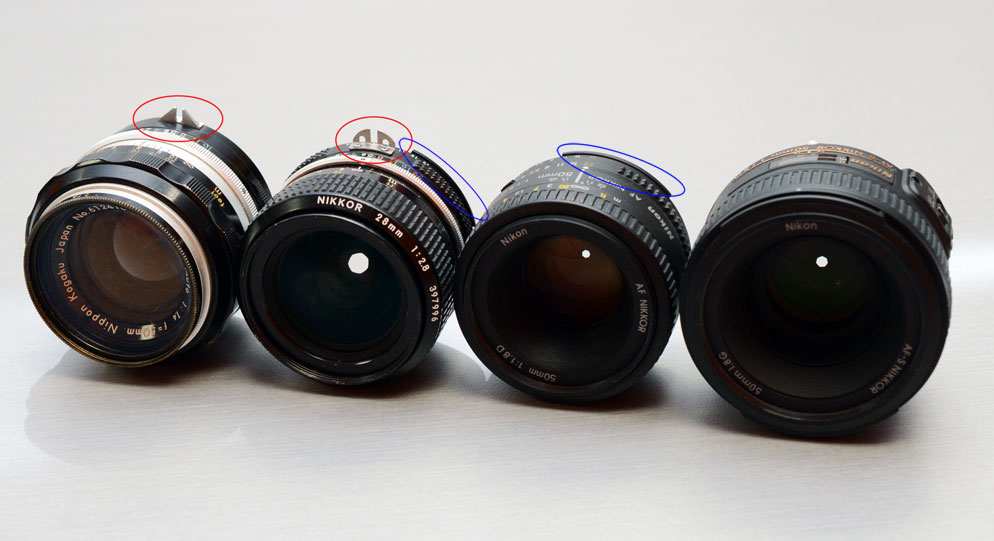
\includegraphics[width=0.75\linewidth]{img/lenses-AI-and-non-AI.jpg}
        	\caption{Nikon objektívek mechanikus rekeszátmérő csatlakozói \cite{Legacy_lenses}}
            \medskip
            \justify Balról jobbra: Nikon AI-előtti objektív, rekeszátmérő csatlakozó pirossal bekarikázva; Nikon AI objektív,  rekeszátmérő csatlakozó cipő pirossal bekarikázva, rekeszátmérő csatlakozó gerinc kékkel bekarikázva; Nikon AF-D objektív, rekeszátmérő csatlakozó gerinc kékkel bekarikázva; Nikon AF-S objektív nem kommunikál rekeszátmérő információt mechanikusan.\cite{Legacy_lenses}
        	\label{fig:Exposure_coupleing}
        \end{figure}
    \end{itemize}
\end{itemize}

Az objektív által a fényképezővázon mechanikusan állított értékek:
\begin{itemize}
    %\item Objektív gyújtótűvolsága, AI-típusú objektíveken %\cite{Nikon_naming_convention}
    \item Objektív jelenleg beállított rekeszátmérője. \cite{Lens_naming}
    \item Objektív maximális rekeszátmérője. \cite{Lens_naming}
\end{itemize}

\subsubsection{Csavar alapú autófókusz}

Az objektíveknél, amelyek ezt a mechanizmust használják, "nem lehet az autófókuszt üzemeltetni, kivéve ha egy beépített fókuszmotorral rendelkező digitális vagy film SLR kamera van használva." A fókuszálási sebesség attól függ, hogy a vázba épített fókuszmotor, milyen sebességgel képes forgatni a (\ref{fig:F100_AF_csavar}) képen látható csavarfejet, ami a (\ref{fig:AF_csavar}) képen látszódó csavart hajtja meg.
% there can be no autofocus operation unless a digital or film SLR camera with the autofocus motor built-in to the camera body is used

\begin{figure}[H]
	\centering
	\includegraphics[width=0.5\linewidth]{img/F100_AF_csavar.jpg}
	\caption{Nikon fényképezőgépvázon található AF fókuszáló csavar}
	\label{fig:F100_AF_csavar}
\end{figure}

%\begin{figure}[H]
%	\centering
%	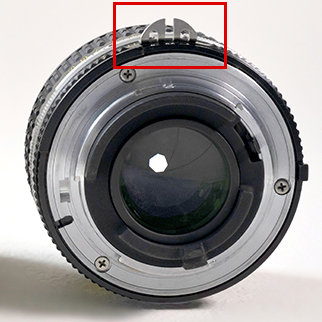
\includegraphics[width=0.5\linewidth]{img/Nikon-AI-bütyök.jpg}
%	\caption{Nikon AI objektív csatlakozása. Rekeszátmérő csatlakozó bekeretezve.\cite{Nikon_CPU}}
%	\label{fig:AI_back}
%\end{figure}

\begin{figure}[H]
	\centering
	\includegraphics[width=0.5\linewidth]{img/F100_bajonett.jpg}
	\caption{Nikon F100-as fényképezővázon található F bajonettcsatlakozás}
	\label{fig:F_bajonett}
\end{figure}

\subsubsection{Mechanikus autómatikus diafragma}
A legtöbb Nikon objektíven ilyen autómatikus diafrámmal rendelkezik.
A (\ref{fig:G_rekeszkar}) képen látható álláskapcsolót egy rugó (amennyiben a álláskapcsolót más meg nem mozdítja) a zárt pozíció felé tolja.
A fókuszálás során a álláskapcsolót egy, a fényképezőgépvázon található kar, a nyílt pozícióba mozgatja.
A kép készítésekor ez a kar úgy mozdul, hogy az álláskapcsoló szabadon a zárt pozícióba tudjom kerülni, a rugó nyomásának köszönhetően.
Eközben a rekeszátmérőért felelős lamellák addig záródnak össze, amíg meg nem állítja őket az objektív belső mechanikája, ami a fényképkészítő gomb lenyomása előtt került beállításra.

Az álláskapcsoló addig marad zárt állásban, amíg a fényképezőgép kéri, ezt követően a kar visszaviszi a kapcsolót a nyílt állásba, és várja a további utasításokat.
A zárt állapot több kép elkészítésén át is fennmaradhat, amennyiben azok elég gyorsan követik egymást.

\begin{figure}[H]
	\centering
	\includegraphics[width=0.5\linewidth]{img/Nikon_17-55_zart.jpg}
	\caption{Nyugalmi állapotban a G jelölésű objektív rekesze zárva van.}
	\label{fig:17-55_zart}
\end{figure}

\begin{figure}[H]
	\centering
	\includegraphics[width=0.5\linewidth]{img/Nikon_17-55_nyilt.jpg}
	\caption{A rekeszátmérő kart elhúzva a rekesz kinyílik.}
	\label{fig:17-55_nyilt}
\end{figure}
\clearpage
\section{NIKON Z BAJONETT}
A nikon Z bajonettcsatlakozás a Nikon tükör nélküli kameráin (MILC) használat objektívcsatlakozás. A csatlakoztatott eszköz és a fényképezőgépváz közti kommunikáció teljes mértékben elktronikusan történik. Itt minimum annyi információ átvitel zajlik, mint a Nikon F bajonett esetében, így az összes F bajonettes kiegészítő irányításához szükséges adatot a Z bajonettes fényképezőgép képes elküldeni és fogadni. A rögzítés az F csatlakozásnál használt módszerekkel történik, azonban dimenzióiban és implementációjában különbözik. "A rendszer nagy objektív foglalata egy 55mm-es belső átmérővel és egy rövid, 16mm-es foglalat-filmsík távolsággal van ellátva (...)."\cite{Nikon_Z}
%The system’s large lens mount features a 55mm inner diameter and short 16mm flange focal distance

\begin{figure}[H]
	\centering
	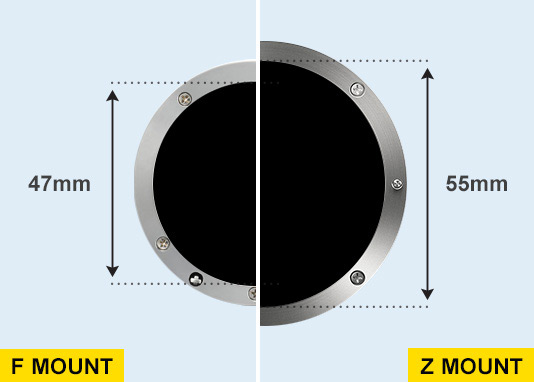
\includegraphics[width=0.5\linewidth]{img/F-mount-vs-Z-mount-illustration.jpg}
    \cite{Nikon_Z}
	\caption{Nikon F (bal) és Nikon z (bal) objektívfoglalatok belső átmérője közti különbség}
	\label{fig:F100_AF_csavar}
\end{figure}
\clearpage
\section{ELEEKTRONIKUS KONTAKTOK ELEMZÉSE}
Bár az elektronikusan közölt információk típusa (pl.: rekeszátmérő) nagyban ismert, hogy pontosan melyik elektronikus kontakt, pontosan milyen módon közli az információt, ismeretlen. Így mind a Z-bajonett mind az F-bajonett elektronikus kommunikációja egy fekete dobozhoz hasonlítható. Ennek a rendszernek a feltárására célszerű megközelítés visszafejtéses módszereket alkalmazni. "A visszafejtés itt úgy van definiálva, mint egy bizonyos hardverhez készült specifikációk létrehozása valaki olyan által, aki nem tartozik az eredeti dizájnerek közé, elsősorban egy egyed vagy egyedek gyűjteményének analizálására vagy dimienziózására alapozva."\cite{Reverse_engineering}
\subsection{Elemek azonosítása}
Első lépésként a konkrét kontaktok által szállított információk jelentéseit kell meghatározni. Ehhez először rögzítenünk kell a kontaktok különböző bemenetére adott reakcióját. Így miközben egy objektív csatlakoztatva van, méréseket végzünk a kapcsolaton. Ezt az alábbi (\ref{fig:jelparosito_UML}) diagrammon látható rendszerrel valósíthatjuk meg. Itt a jel leírásánál fel kell tüntetni az áramerősséget és a feszültséget is, mivel mindkettő tartalmazhat szükséges információt.
\begin{figure}[H]
	\centering
	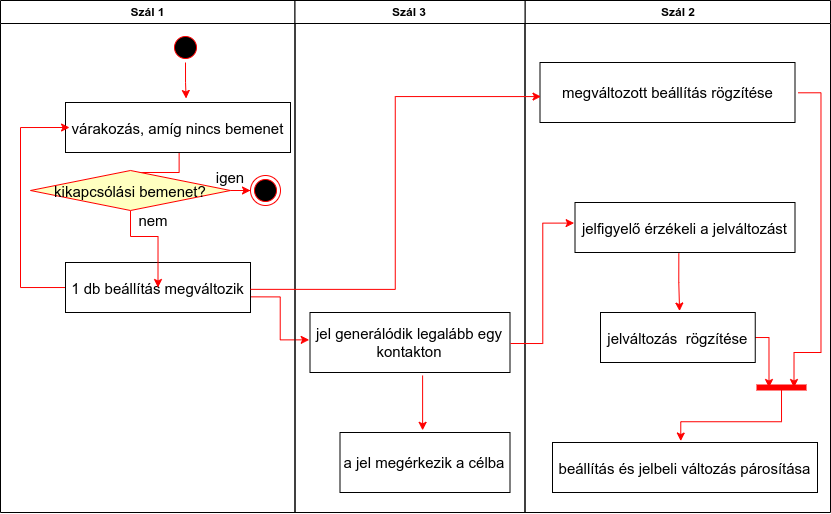
\includegraphics[width=1.0\linewidth]{img/Reverse_2.drawio.png}
	\caption{Nikon F (bal) és Nikon z (bal) objektívfoglalatok belső átmérője közti különbség}
	\label{fig:jelparosito_UML}
\end{figure}
Fontos a bemeneti és a kimeneti (jelek a kontaktokon) változásokat összepárósítani, mivel így a bemenetek alapján rendezve könnyebben meghatározható, hogy mely adatokért mely csatornák felelnek.
\subsubsection{Rögzítőberendezés}
A rögzítőberendezés nem feltétlenül képes minden kontaktot egyszerre felügyelni. Ilyenkor ugyanazokkal a beállításokkal meg kell ismételni a tesztet addig, amíg nem lesz tesztelve az összes kontakt az adott beállítással. Az objektív és a kameratest közé nem juthat be fény, ezért keskeny, alacsony feszültségű kábelekkel kell kivezetni a jeleket a csatlakozások belsejéből. Annak érdekében, hogy az objektív és a kamera ne sérüljön, célszerű egy olcsó makró toldógyűrűt beiktatni a kettő közé, és abba kialakítani a réseket, amiken keresztül a jelet ki lehet vinni a szerkezetből. Miután az eszköz elvégezte a méréseket a jelet továbbítani kell az objektívnek, hogy annak (ha van) válasza is rögzülhessen.
\begin{figure}[H]
	\centering
	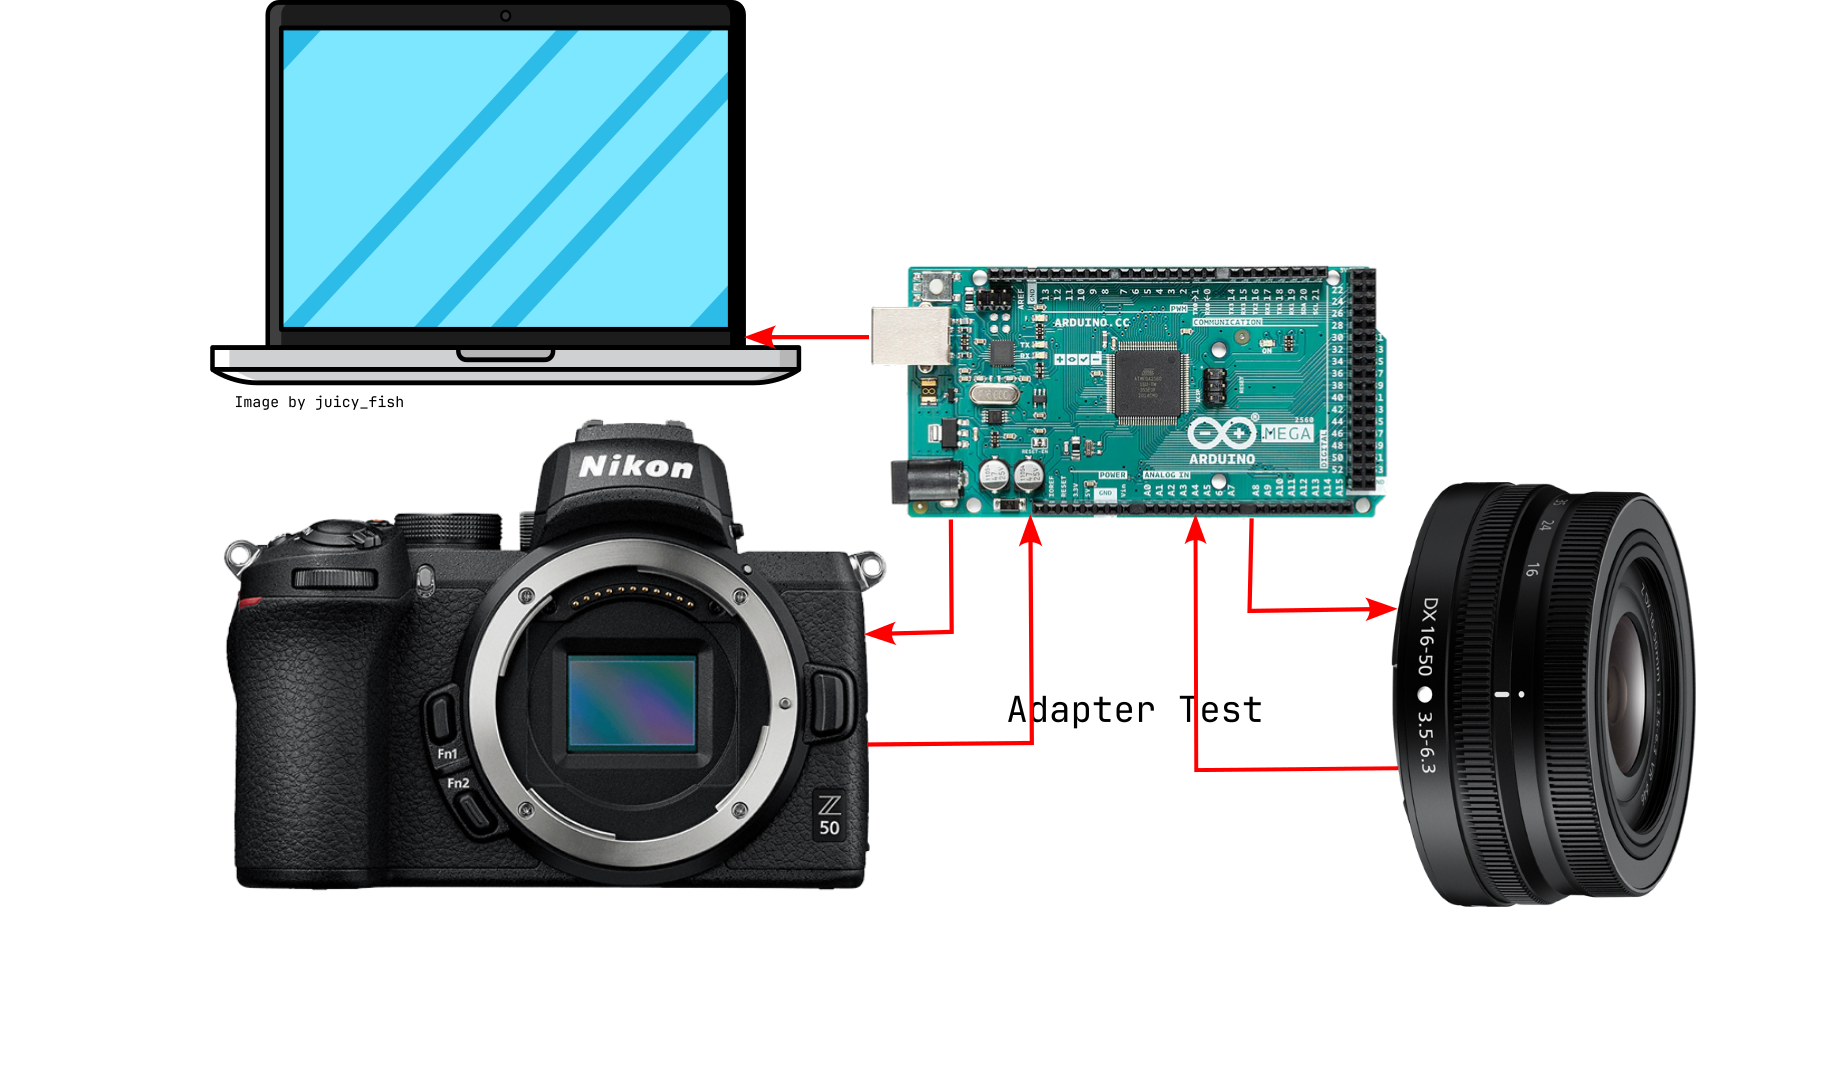
\includegraphics[width=0.9\linewidth]{img/rajz.png}
    \cite{Nikon_Z}\cite{Nikon_Z_16-50}
	\caption{Nikon Z interfész adatrögzítő}
	\label{fig:rogzito}
\end{figure}
\subsubsection{Mintavételezés}
A mintavételezésnek nem sokkal a beállítás megváltozása elött kell kezdődnie, és a jel végeztével le kell állnia. Ezzel látványosan lehet szemléltetni az értékváltozást, és kinyerhetővé válik a jelváltozás szükséges sebessége, valamint a rögzítés megfelelően időzített leállításával elkerülhető a fölösleges feljegyzések generálása, ezzel csökkentve az adatfeldolgozással töltött időt.
\paragraph{Mintavételezési gyakoriság}
Mivel a jelet rögzítésnél az analízis érdekében analógként kezeljük (nem digitális 1 eseket és nullákat rögzítünk, hanem az elektromos jel fentebb említett tulajdonságainak értékeit rögzítjük), de digitálisan tároljuk, ezért meghatározott időközönként kell mintavételezést végeznünk. Ennek a gyakoriságát a Nyquist-Shannon mintavételezési elmélet alapján határozzuk meg. "A Nyquist elmélet leírja, hogy hogyan lehet mintavételezni egy hullámból úgy, hogy ne vesszen el információ."\cite{por2019nyquist} Eszerint a mintavételezési gyakoriságnak a jel legnagyobb lehetséges frekvenciájának kétszeresének kell lennie (\ref{eq:Nyguist})\cite{por2019nyquist}.

\begin{align}
    f_{minta} \geq 2f_{max}
    \label{eq:Nyguist}
\end{align}	
\cite{por2019nyquist}

Ebből következik, hogy egy mintavételezési gyakoriság alapján meghatározható az a frekvencia, aminél kisebb, vagy azonos frekvenciájú jelek veszteség nélkül visszaállíthatóak (\ref{eq:Nyguist_freq}). Ez a frekvencia a Nyguist frekvencia.

\begin{align}
    f_{Nyguist} = \frac{1}{2}f_{max}
    \label{eq:Nyguist_freq}
\end{align}	
\cite{por2019nyquist}

A maximális frekvencia meghatározásához előbb a mintavételező maximális mintavételezési sebességét használva, interpolációval hozunk létre egy függvényt. Ezt elég minden kontakt esetén egyszer elvégezni, azonban több méréssel, és azok egyesítésével megbízhatóbb eredményt kapunk. Ilyenkor valószínűleg a szükségesnél nagyobb a mintavételezési frekvencia, ezért az interpolációt el lehet végezni. A függvény csúcsai közti idő felhasználásával határozzuk meg az $f_{max}$ frekvenciát. Ezt a (\ref{eq:csucsok}) képlettel kaphatjuk meg. A csúcsokat az g(idő) függvény deriválásával, a deriváltfüggvény zérushelyeinek meghatározásával, és a kapott helyek közül a pozitív függvényértéket felvevők kiválasztásával érdemes elvégezni.

\begin{align}
    f_{max} = \frac{1}{min^{n - 1}_{i = 1}(|t_{i} - t_{i + 1}|)}
    \label{eq:csucsok}
\end{align}	
\small Ahol $n$ a csúcsok száma és $t \in T$ a csúcs rögzítésének ideje.

Egy beállítással több mérést is kell végezni, így csökkentve az esélyét annak, hogy egy vagy több meghibásodásnak köszönhetően rossz konklúzióra jussunk. Az ideális tesztek számát a méréseket végző türelme, és a kapott értékek közti különbségek alapján lehet meghatározni.

\subsubsection{Adatok rendezése}
Hogy könnyebben értelmezhetőek legyenek az összegyűjtött adatok, azokat szűrni és egyesíteni kell. Az alábbi két folyamat elsősorban az összegyűjtött adatok elemzésére szolgál, nem használatosak az adapteren. Ez a módszer nem növeli annyival az adatok pontosságát, hogy az adapteren megérje alkalmazni.
\paragraph{Hibás adatok szűrése statisztikai módszerekkel} A kapott adatokból létrehozunk egy 99\%-os konfidenciaintervallumot, és az azon kívül eső elemeket eltávolítjuk a minták közül úgy, hogy a helyükre a kettő szomszédos érték étlagát írjuk be. Ezáltal a mintavételezési sűrűség nem változik.
\paragraph{Hibás adatok szűrése zajforrás megszüntetésével} Maga a mérőeszköz is képes zajt generálni. Ennek érdekében használjuk a \ref{ADC_noise} kifelytett eljárást.
\paragraph{Zaj szűrése a jel dekompozíciójával} Bizonyos frekvenciákat eltávolítva tisztább, könnyebben elemezhető jelet kapunk. Ehhez egy metódus a \ref{OMP} szekcióban kifejtett módszer.
\paragraph{Összefésülés több mérés esetén}
Mivel az adatrögzítés a minden feljegyzés esetében, a beállításváltozáshoz képest ugyanakkor kezdődik és ér véget, valamint a mintavételezési gyakoriság megegyezik, ezért az egy beállításhoz tartozó adatokat a mérés kezdése óta eltelt idő alapján csoportosíthatjuk. A fenti szűrés elvégzése után a több mintából egyet alakítunk ki úgy, hogy egy ilyen kategóriába tartozó adatoknak az átlagát vesszük, és az így keletkezett feljegyzésből állítjuk vissza az eredeti függvényt. Ez az adapteren nem értelmezhető, mivel csak egy adatfolyammal tud dolgozni, a jelenlegi mérések alapján.
% ide le kellene írni, hogy hogyan kell visszaállítani.

\subsection{Jelek átalakítása}
Az adathalmaz kialakítása után értelmezni kell a kapott függvényeket, és azokból a bemenet alapján kinyerni az adatokat
\subsubsection{Analóg és digitális jelek elkülönítése}
Elektronikus úton két féle képpen lehetséges adatokat továbbítani. Az elektromos jel lehet digitális vagy analóg. A fenti adattranszformációk elvégzése után a függvényt vizualizálva könnyen megállapítható annak típusa következő módon. Amennyiben a függvény értéke két érték között váltakozik, azokat elérve ezeket az értékeket egy bizonyos ideig tartják, akkor ez egy négyzetfüggvény és digitális jelre utal. Amennyiben a jel több értéket is felvesz, valamint hullámossága nagyobb, akkor a jel analóg.

\begin{figure}[H]
	\centering
	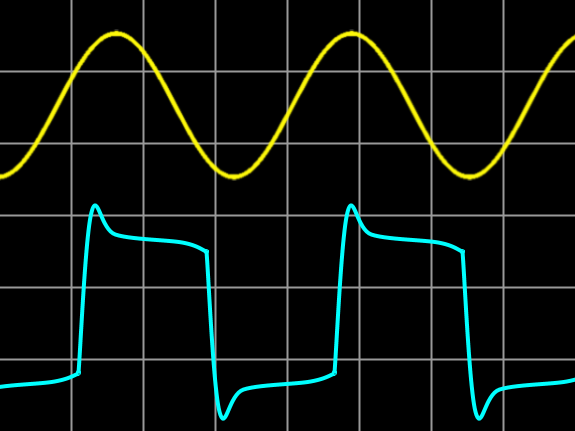
\includegraphics[width=0.5\linewidth]{img/oszcilloskóp.png}
    \cite{digital_vs_analog}
	\caption{Analóg (fent) és digitális (lent) az oszcilloskópon}
	\label{fig:oscilloszkop}
\end{figure}

\subsubsection{Analóg jelek transzformálása}
\paragraph{Analóg-Analóg kapcsolat}
Az ilyen típusú jelek pontos jelentését nehéz meghatározni. Ezért amennyiben az adott funkciót mind a Z és az F oldalon analóg jelek látják el, akkor az egyik oldalról kapott mintákon lineáris transzformációt végzünk úgy, hogy a másik oldal interfészének megfeleljen.
\paragraph{Analóg-Digitális kapcsolat}
Ebben az esetben kötelező értelmezni az analóg jelet. Ezt úgy lehet megtenni, hogy az ismert bemenettel asszociáljuk az adatgyűjtés során kapott analóg függvényt. Amennyiben a kapott analóg függvény eléggé hasonlít (a bemenet értékének, annak változásának, valamint a mintafügvény értékének, annak változásának, különbsége határártéken belül van), akkor kimeneti digitális jel az analóg jellel asszociált digitális jelet adja tovább. Amennyiben a jelet digitálisról kell analógra váltani, akkor a kimeneten a digitális jellel asszociált függvényt kell megjelentetni.

\subsubsection{Digitális jelek analizálása és transzformálása}
A digitális jelet elöször demodulárni kell (analógból digitálissá alakítani), miután megállapítottuk a moduláció módját az analóg forrás vizsgálatával. Amennyiben ezt támogatja a mikrokontroller bemenete, annyiban nem szükséges további szoftveres feldolgozást végezni az analóg jelen, máskülönben a demodulációt be kell iktatni a mikroprocesszoron futtatott szoftverbe. Ezt követően a bemenetből és az ipari szabványokból kiindulva dekódolni lehet az adatokat. Azonban ez a legtöbb esetben nem szükséges, mivel a cél a két interfész közti adatmegfeleltetés. Így elég egy hasítótábla segítségével kikeresni digitális jelbemenetnek megfelelő kimeneti adatláncot, és azt továbbküldeni. Amennyiben a két adatlánc közt matematikai összefüggés is leírható, akkor azt érdemes használni a transzformációra, a memóriaigény csökkentése, és a gyorsabb reakció érdekében.
\clearpage
\section{IMPLEMENTÁCIÓ}
Ez az egység végzi az adatok feldolgozását, a jelek átalakítását.
Ezt a szerepet egy Arduino Mega 2560 Rev3 egység fogja ellátni\cite{parmar2017design}.\\Ennek az eszköznek az előnyei:
\begin{itemize}
    \item Alacsony energiafogyasztás (7-12V, 1A)\cite{arduino_docs}
    \item Nagy mennyiségű analóg bemenet (16db láb)\cite{arduino_docs}
    \item Nagy mennyiségű digitális ki és bemenet (54db láb)\cite{arduino_docs}
    \item PWM láb az analóg jelgeneráláshoz (15db)\cite{arduino_docs}
    \item 9V-os akkumulátorral képes üzemelni \cite{arduino_docs}
    \item Részletes dokumentáció, és sok segédanyag
\end{itemize}
Hátrányai:
\begin{itemize}
    \item Gyenge processzor (ATmega2560 16 MHz)\cite{arduino_docs}
    \item Kevés memória (8KB SRAM, 256KB FLASH, 4KB EEPROM)\cite{arduino_docs}
    \item Tisztán analóg kimenet hiánya.
\end{itemize}
\subsection{Jeltranszformáció}
Azoknál az átalakításoknál, ahol az interfésznek legalább az egyik felén digitális jel van, ott használatos ez az eszköz.
\subsubsection{Digitális-Digitális transzformáció}
Ebben az esetben a be és kimeneteket a Digitális be, és kimenetekre kell kötni. A transzformációt a bemeneti jel fogadása után elvégzi az eszköz, és a kapott adatokat a kimeneti digitális kapcsolaton továbbküldi.
\subsubsection{Analóg-Digitális transzformáció}
Ebben az esetben az egyik analóg bemenetre rákötjük az analóg interfészt, a digitális kimenethez pedig a kimeneti, digitális intefészt kötjük. Miután az 5.2.2-es szekcióban ismertetett módon létrehozzuk a digitális adatokat, azokat a kimeneti digitális tűn továbbküldjük.
\subsubsection{Digitális-Analóg transzformáció}
Ilyenkor a digitális bemenet egy digitális bemeneti tűre van kötve, az analóg kimenet pedig egy PWM tűn fog megjelenni. Az 5.2.2-es szekcióban ismertetett eljárás alapján kiválasztjuk a függvényt, majd annak felhasználásával létrehozunk egy olyan modulált jelet a PWM csatornán, amely azt a függvényt reprezentálja. Ezt a jelet küldjük a kimeneti csatlakozásra.
\subsubsection{Analóg-Analóg transzformáció}
A bemenet ilyenkor az egyik analóg bemeneti tűre van rákötve, a kimenet pedig egy PWM tűre. Az analóg bemenetből az 5.2.2-es szekcióban ismertetett módszerek segítségével kell előállítani a kimeneti függvényt, majd azt a \textbf{Digitális-Analóg transzformáció} bekezdésben ismertetett módon kell a PWM kimeneten megjelentetni. Ahol a kettő jel között matematikai, és nem logikai kapcsolat van, ott az alábbiakban ismertetett megoldás jobb eredményeket adhat.
\subsection{Analog-Digital Converter - ADC (Analóg-Digitális Konverter)}
A mikrokontroller analóg lábain a beolvasásra kerülő jeleket a rajta található ATmega2560 processzor\cite{arduino_docs} Analóg-Digitális konvertere 10-bit es egész számokká alakítja\cite{ATmega_processor_datasheet}. Az így kapott szám azt mutatja, hogy a beolvasott érték az analóg lábak határértékei (0V és 5V) között hol helyezkedik el. Ebből feszültséget a kövekező formulával számolhatunk:
\begin{align}
    U(x) = \frac{5Vx}{1023}
\end{align}
\small (1023 a legnagyobb 10-bit-en reprezentálható érték)

\subsection{Áramforrás}
Áramforrásként a mikrokontroller dokumentációjában említett USB tápellátás használatos a prototípus fejlesztésekor.
Amennyiben a váz objektívtápellátása stabil 5V, vagy 7-12V, ezek használatosak.\cite{arduino_aram}
Mivel az 5V egy elterjedt tápellátási forma, és a Nikon F csatlakozás is ezt hasznélja objektítápként, ezért ez nagy valószínűséggel alkalmazható.
Ilyenkor el lehet kerülni egy akkumulátor rendszeres cseréjét.
Ha a tápellátás nem 5V, de 7-12V közé esik, akkor azt csatlakoztatni kell a mikrokontroller VIN lábára.
Ennél ügyelni kell arra, hogy nem rendelkezik fordított polaritás védelemmel, ezért a bekötést megfelelően kell elvégezni.\cite{arduino_docs}
Amennyiben a feszültség stabil 5V, a feszültség az elektromos áram az eszköz számára megfelel, így egyenesen az 5V-os bemeneti lábra köthető.

Amennyiben a Z csatlakozás tápfeszültsége(i) nem egyeznek meg az F csatlakozáséval, erősítők, ellenállások segítségével kell azt az F csatlakozás tápfeszültségével egyenlővé tenni.

\subsection{Programozása}
A mikrokontroller programozásához telepíteni kell az Arduino szoftvert a programozó számítógépére.
A mikrokontrolleren nem lehet azt programozni.
A programozáshoz elérhető egy telepíthető IDE és egy webes verzió is.
A kettő közül a telepíthető verzió használata ajánlott.
Ezt követően az Arduinót a számítógéphez csatlakoztatjuk USB-n keresztül, így lehetőség nyílik a mikrokontrollerre programot feltölteni. \cite{monk2023programming}
Ilyenkor az arduinokhoz készített programozási nyelvet használjuk.
Ezzel a legegyszerűbb programozni ezeket az eszközöket, mivel az IDE a hardver köré épült (pl.: GUI vezényli az áttöltést, fordítást).
A nyelv a C++ nyelvre alapszik, így a legtöbb C++-ban írt program az arduino fordítójával is a várt eredményt produkálja.
A nyelv nem garantálja a memóriabiztonságot, aminek következtében a szoftver abnormálisan érhet véget. Ennek elkerülése érdekében kettő lépést is meg lehet tenni.
\begin{itemize}
    \item A dinamikus memóriaallokációk számának csökkentése a programban.
    \item Memóriabiztos rendszerprogramozási nyelv használata.
\end{itemize}
A második kritérium megvalósítására ideális programozási nyelv a Rust, amely egy memóriabiztonságos nyelv, azonban egy alapértelmezett projekt felépítése nem alkalmas az arduinón történő futtatásra.
\subsubsection{Hardver Absztrakciós Réteg}
% all the software that is directly dependent on the underlying HW.
"Hardver absztrakciós rétegként (HAL) definiálható minden olyan szoftver, amelynek közvetlen függősége a hardver."\cite{yoo2003introduction}
Ilyen az Arduino rendszerekhez kifejlesztett hardver absztrakciós réteg került felhasználásra.
Ennek a rétegnek köszönhetően olvashatóbb kód írható, assembly elkerülésével, és az így kapott kód minimális módosításával a program más hardveren futtathatóvá tehető.\cite{yoo2003introduction}
Egy elterjedt Rust-hoz készített ilyen eszköz az \textit{arduino-hal}.\cite{arduino_hal}
Ennél fontos 2025-01-01 Rust toolchain-t támogató verzió használata fordítóhibák elkerülésé végett.\cite{avr_compiler_bugs}

%\subsubsection{Dedikált áramkörök}
%Ezeket az \textbf{Analóg-Analóg} transzformáció során kell használni a gyorsabb jelátadás érdekében, ahol lehet. Itt a megfelelő matematikai műveleteket megvalósító áramkörök segítségével kell elvégezni a jelátalakítást. Ehhez szükséges a két jel közti matematikai összefüggés, összefüggések ismerete. Ahol ez a feltétel nem áll fenn, ott a fentebb leírt mikrokontrollerrel történő megoldást kell alkalmazni. A lehető legtöbb helyen passzív áramköröket kell alkalmazni, viszont ahol elkerülhetetlen, ott külső áramforrásra kell támaszkodni. Ekkor a prototípus fejlesztésénél a mikrokontrollertől független, a kész eszköznél lehetőleg a mikrokontroller által használt áramforrás használatos. Hasonló rendszerek használatával a fényképezőváz által nyújtott áramforrást el lehet osztani a mikrokontroller és az objektív között.

%\subsubsection{AF Autofókuszmotor}
%Ez által valósul meg az AF és AF-D objektíveken az Autófókusz. Ennek érdekében a mikrokontroller értelmezi a váz által küldött autófókuszinformációt (amely valószínüleg csak az irányt tartalmazza), és az alapján mozgat egy léptető motort. Amennyiben a csatlakoztatott objektívnek nem ad autofókusz utasításokat a váz, annyiban az adapternek olyan hamis információkat, azonosítási adatokat kell a váznak küldenie, amelyek hatására az megkezdi azok küldését. "Egy léptetőmotor egyszerre egy lépést tud mozdulni a hagyományos motorokkal ellentétben, amik folyamatosan mozognak."\cite{parmar2017design} Ezt a technológiát Nikon objektívek autofókuszálására is használják az AF-P jelölésű objektíveken \cite{Nikon_AF} a precizitásuk és sebességük miatt. "Ha parancsot adunk egy léptetőmotornak, hogy tegyen meg egy bizonyos számú lépést, akkor inkrementálisan annyi lépést mozog és megáll. "A léptető motor ezen alap természetének köszönhetően, általában alacsony költségű, nyílt hurkú pozíció irányitási rendszerekben használatosak. A nyílt hurkú irányítás azt jelenti, hogy nem igényel visszacsatolási információt a pozícióról." \cite{parmar2017design} Mivel nem tudjuk minden AF objektív jelenlegi fókusztávolságát\cite{Nikon_AF}, ezért egy ilyen nyílt hurokkal dolgozunk, tehát egy ilyen típusú motor ideális választás a fókuszcsavar pozícionálására. %https://www.adafruit.com/product/4411
% A stepper motor can moves one step at a time, unlike those conventional motors, which rotate continuously
% If we give command a stepper motor to move some exact number of steps, it rotates incrementally that many number of steps and stops. Because of this basic nature of a stepper motor, it is generally used in low cost, open loop position control systems

%\subsubsection{Váz oldali autofókuszcsavar}
%Ennek az elemnek két egyszerű beszerzési módja van. A 3D-s nyomtatás, valamint egy ilyen rendszerrel rendelkező kameravázból való kiszerelés. Az utóbbi biztosabb működést ad, míg az előbbivel több példányhoz juthatunk hozzá, a megfelelő dizájn elkészítésének az árán. Ezt  a csavart egy rugó nyomja ki az adapterből, annak érdekében, hogy az objektívek, amelyek ezt nem használják is csatlakoztathatóak legyenek. Emiatt a szárán lévő fogaskeréknek olyannak kell lennie, hogy amikor mozog, akkor is csatlakoztatva maradhasson a léptetőmotorral, amivel fogaskerekek kötik össze.

%\subsubsection{Adaptertest}
%Az adapter két bajonettzárat összekötő testének a megfelelő távolságra kell eltartania az F bajonettes objektívet a Z bajonettes váztól, annak érdekében hogy az objektív a specifikációinak megfelelő intervallumon tudjon fókuszálni. A piacon található adaptereket nehéz módosítani, ezért 3D-s nyomtatással, szabadon elérhető és (ahol megfelelő nem található) modellek alapján készülnek el az adaptertestek. Három adaptertesttet kell elkészíteni: egy adaptertestet, amely a kettő különvöző csatlakozóra illeszkedik az FTZ adapterhez, és egy-egy makrógyűrűt, amelyekkel a natív vázak és objektívek közötti kommunikáció kerül reögzítésre. Mindegyik féle adaptertest oldalán jukaknak kell lenniük, itt lesznek kivezetve a jeleket vezető szálak, hogy a mérőeszkozzel hozzájuk lehessen férni. Ezen kívül, még hozzájuk kell adni a csatlakozónál kontaktokat tartó elemeket is.
\clearpage
\section{ZAJSZŰRÉS ÉS JELKIEMELÉS}
"A zaj egy kéretlen jelek egy típusa.[...] Az adatgyűjtési folyamat során a zaj a jelekben perzisztens.[...] 
Még az analóg-digitális átalakítás is zajt ad az átalakított jelhez. 
A konverter minőségétől és a jel felhasználásától függően ennek jelentős hatással lehet."\cite{noise_reduction_omp}
Annak érdekében, hogy egyszerűbb legyen egyezéseket találni az analóg bemenetek, és az azokhoz eltárolt minták között.
Ezek a szűrők az elemzési fázisban is jól használhatóak, így könnyebb automatizált eszközökkel mintákat találni a jelekben.

\subsection{Digitális zaj csökkentése} \label{ADC_noise}
"Tipikus forrásai a magas frekvenciájú zajnak, amely hatással van az áramkörökre és elektronikus rendszerekre: digitális logika, kapcsoló tápegységek, elektrosztatikus kisülések, motorok és relék, [...]. 
A digitális zaj valósszínűleg a legelterjettebb zajforrás az elektronikus rendszerekben."\cite{smith1992high}
Az Arduino Mega 2560 az ADC pontosságának növeléséhez nyújt egy "ADC Noise Reduction" alvási módot \cite{arduino_at_mega_datasheet}. 
"Az ADC képes Alvó módban üzemelni, de ehhez az ADC-nek a dedikált ADCRC-r kell használnia órajel forrásként. 
Amikor az ADCRC van kiválasztva órajel forrásként, az ADC hardver vár még egy instrukciós ciklust ($T_{CY}$) mielőtt megkezdi a konverziót. 
Ez megengedi, hogy a SLEEP instrukció végre legyen hajtva, amely csökkentheti a rendszerzajt a konverziós folyamat során."\cite{ATmega_processor_datasheet}

\subsection{Zajcsökkentés DCT és DSC szótárakon alapú OMP algoritmussal} \label{OMP}

Ez a módszer a fehér nagyjából 34dB-el képes csökkenteni, miközben visszaállítja torzításmentesen az eredeti jelet.\cite{noise_reduction_omp}
Az eljárás "a feldolgozott jelből diszkrét koszinus transzformációval és diszkrét szinusz transzformációval létrehozza annak a ritka reprezentációját. Az ortogonális egyezésre törekvés algoritmusa rekonstrukciós algoritmusként van használva, hogy a zaj nélküli jel bázisait megtaláljuk [...]."\cite{noise_reduction_omp}
A ritka reprezentáció a következő lineáris kombinációval képes a jelet reprezentálni:
\[x[n]=\sum_{m=1}^{M}D[n,m]\alpha[m]+r[n]\]
ahol $x[n]$ egy $x \in \mathbb{R}^{N \times 1}$ jel n-edik mintája, $D[n,m]$ az n-edik mintája az m-edik oszlopnak (atom) egy $D \in \mathbb{R}^{N \times M}$, $a[m]$ az m-edik együtthatója egy $a \in \mathbb{R}^{M \times 1}$ritka vektornak (van nem 0 eleme) és $r[n]$ az n-edik mintája a visszamaradó $r \in \mathbb{R}^{N \times 1}$ reprezentációnak.\cite{noise_reduction_omp}

\paragraph*{OMP(ortogonális egyezésre törekvés) algoritmus}
"Egy mohó algoritmus, amely használható jelvisszaállításra hiányos együtthatókból tömörített érzékelésnél."\cite{noise_reduction_omp} Esetünkben a jel dekompozíciójára használjuk.

% \begin{algorithm}
%     \caption{OMP}\label{alg:cap}
%     \begin{algorithmic}
%         \Require
%         \Ensure
%         \While {$\neg STOP\_CRITERION$}
%             \State $j++$
%             \State $i = \underset{m=\{1,...,M\}}{argmax}| \langle r, D \rangle |$ \Comment{A maximum abszolút értékű belső szorzata a \newline visszamaradó jelnek ($r$) és a $D$ szótár összes $d_m$ atomjának.} % https://mathworld.wolfram.com/AngleBracket.html
%             \State $U_{j}=[U_{j - 1} \cup i]$
%             \State $D_{j}=[D_{j - 1} | d_{i}]$
%            \State $\underset{\alpha}{min} \norm{x - D_{j}\alpha_{j}}_{2}^{2}$
%           \State $r_{j} = x - \tilde{D}_{j}\alpha{j}$ \Comment{$\alpha = \tilde{D}_j^{\dagger}x$ ahol $\dagger$ Moore–Penrose pseudo-inverz mátrixot jelez}
%        \EndWhile
%        %\Return \alpha_{j}, U_{j}, r_{j}
%    \end{algorithmic}
%\end{algorithm}\cite{noise_reduction_omp}
% Ahol: 
% $x$: dekompozálandó jel
% $D$: szótár, amely regisztrálja a kiválasztott atomot
% $STOP_CONDITION$: Leállási feltétel
% $r$: Visszamaradó jel.(Inicializálásnál ($r_0$) az eredeti jel, ekkor $D_0$ és $U_0$ is üres)
% $U$: index vektor, amely a kiválasztott atom indexét regisztrálja.
% $j$: Elleniterátor. (Kiinduláskor 0)
% $\tilde{D}$: Atomok részmátrixa.
A ritka reprezentáció megtartása érdekében $M > N$ nek igaznak kell lennie és a szótárban legalább $N + 1$ atomank kell lennie.
A diszkrét fourier függvény complex része elkerülése érdekében a DCT és a DST algoritmusokat használjuk. Ezek eredményéiből jön létre a szótár: \[D = [C|S]\]
A koszinuszok a DCT-II transzformáció alapján: \[C[n, k] = \beta_c \cos[\frac{\pi k (2n + 1)}{2N}]\]
A szinuszok a DST-II transzformáció alapján: \[C[n, k] = \beta_s \sin[\frac{\pi (k + 1) (2n + 1)}{2N}]\]
Ahol 
\begin{equation}
    \beta_c =
    \begin{cases}
        \sqrt{\frac{1}{N}}, n = 0\\
        \sqrt{\frac{2}{N}}, 1 \leq n \leq N - 1
    \end{cases}
\end{equation}
\begin{equation}
    \beta_s = 
    \begin{cases}
        \sqrt{\frac{2}{N}}, 0 \leq n \leq N - 2\\
        \sqrt{\frac{1}{N}}, n = N - 1
    \end{cases}
\end{equation}
$n = {0, 1,..., N - 1}$, $k = {0, 1,..., N - 1}$ és $N$ a jelminták száma. Ezek alapján a ritka reprezentáció:
\begin{equation}
    x[n] = \sum_{p=1}^N C[n,p]\alpha_c[p] + \sum_{q=1}^N S[n,q]\alpha_s[q] + r[n]
\end{equation}
Ahol $\alpha_c \in \mathbb{R}^{N \times 1}$ a koszinuszok, $\alpha_s \mathbb{R}^{N \times 1}$ pedig a szinuszok együtthatói amik a $C \in \mathbb{R}^{N \times N}$ és a $S \in \mathbb{R}^{N \times N}$ mátrixokhoz tartoznak. A szótárban $2N$ atom lesz.\cite{noise_reduction_omp}
\\
\begin{algorithm}
    \caption{OMP zajcsökkentés}\label{alg:cap}
    \begin{algorithmic}
        \Require $C, S, x, STOP\_CRITERION$
        \Ensure $r_0 = x, D_0 = {}, j = 0$
        \While {$\neg STOP\_CRITERION$}
            \State $j++$
            \State $i = \underset{m=\{1,...,M\}}{argmax}(\sqrt{\langle r_{j-1}, C_m \rangle^2 + \langle r_{j-1}, S_m \rangle^2})$ \Comment{$\langle \bullet , \bullet \rangle$ skalárszorzat} % https://mathworld.wolfram.com/AngleBracket.html
            \State $U_{j}=[U_{j - 1} \cup {i, N + i}]$
            \State $D_{j}=[D_{j - 1} | {C_{i}, S_i}]$
            \State $\alpha = \tilde{D}_j^{\dagger}x$ ahol $\dagger$
           \State $\underset{\alpha}{min} \norm{x - D_{j}\alpha_{j}}_{2}^{2}$
          \State $r_{j} = x - D_{j}\alpha{j}$
       \EndWhile
       \State \Return $\alpha_{j}, U_{j}, r_{j}$
   \end{algorithmic} \cite{noise_reduction_omp} 
\end{algorithm}
\\
Ahol: \\
$x$: dekompozálandó jel. \\
$S$: Szinusz komponensek. \\
$C$: Koszinusz komponensek. \\
$D$: Szótár, amely a $[C|S]$ mátrixból áll. C és S elemeknek párban kell lenniük (ugyan akkora az elemszámuk).\\
$STOP_CONDITION$: Leállási feltétel. \\
$r_j$: Visszamaradó jel a j-edik iterációnál.(Inicializálásnál ($r_0$) az eredeti jel, ekkor $D_0$ és $U_0$ is üres). \\
$U_j$: A j-edik iterációnál kiválasztott atom indexek halmaza. \\
$j$: Elleniterátor. (Kiinduláskor 0) \\
$\tilde{D}$: Atomok részmátrixa. \\

\paragraph{Megállítási feltétel}
A megállítási feltételhez, egy a szimulált lehűtésnél is alkalmazható módszert használunk.
Ennek alapján akkor állítjuk le az iterációt, ha a az algoritmus energiaszintje elért egy minimumot. Ezt az OMP esetében az alábbiak szerint becsüljük meg:
\begin{equation}
    E_m = \sqrt{\frac{\alpha_m^2 + \alpha_{N + m}^2}{2N}}
\end{equation}
Az $E_min$ értéke fehér zaj esetén meghatározható annak a konstans teljesítményspektrum sűrűsége miatt.
Viszont a módszer miatt az energiaszint elérheti a minimumot, de a megoldás még hullámzik.
Ennek elkerülése érdekében, csak akkor érjen véget a ciklus, ha legalább már kettő egymás utáni megoldás energiaszintje a határérték alatt van.\cite{noise_reduction_omp}
\clearpage
\section{ÓRA}
\input{chapters/8_Óra}
\clearpage
\section{MEGSZAKÍTÁSOK}
\[insert def here\]
\subsection{Megszakítások engedélyezése}
% avr_device::interrupt::enable
Megszakítások használatához először azok bekapcsolása szükséges. Ha a megszakítások nincsenek bekapcsolva, akkor a megszakításokhoz rendelt függvények nem kerülnek meghívásra.

\subsection{Egyedi megszakítás függvény}
A megszakításokhoz csak olyan globális függvények rendelhetőek, amelyeknek nincsenek bemeneteik. Emiatt, minden a függvény lefutásához szükséges külső változónak globálisnak kell lennie.
Így a függvény bemenetként fogadhat változókat és módosíthatja is azokat függvényargumentumok nélkül. Ennek a technikának a használatával válik lehetségessé többek között az óra túlcsordulás számlálójának megvalósítása is az \ref{ora}-as számú szekcióban. 

\subsection{Konkurencia}
Az MCU csak egy maggal rendelkezik \cite{ATmega_processor_datasheet}, ezért a programok párhuzamos végrehajtása nem lehetséges.
Azonban a programrészletek konkurens végrehajtása továbbra is lehetséges akkor, ha egy (vagy több) megszakítás meghívódik.
Ilyenkor a fő program végrehajtása fel lest függesztve, és a megszakítások a prioritási sorrendjüknek megfelelően végrehajtásra kerülnek \cite{ATmega_processor_datasheet}.
Emiatt a program szekvencialitása nem garantálható, és egyes adatstruktúrák nemkívánatos sorrendben történő módosítása hibás programhoz vezethet.

\subsubsection{Kölcsönös kizárás}
Kölcsönös kizárással garantálhatóvá tehető, hogy a program a megfelelő sorrendben kerül végrehajtásra.
% cite avr hal docs
A HAL tartalmaz egy ilyen eszközt, amely egy "kritikus szekciók" alapú megvalósítás.
Segítségével garantálható, hogy egy adott szakasz végrehajtása során nem kerül egy megszakítás sem végrehajtásra.
\clearpage
\section{Naplózás}
\label{sec:naplozas}
\subsection{Felhasználási területek}
Naplózás szükséges az eszköz által érzékelt adatok gyűjtésére a protokoll felderítési fázisban.
Emellett segíthet a különböző hibakeresési folyamatokban, ha a program jelezni tudja, hogy éppen mit csinál, milyen hibákba ütközött.

\subsection{Naplózó kimenet: USART}
Az Arduino nem rendelkezik képernyővel. Látható kimenetként egyedül beépített LEDekkel rendelkezik.
Lehetséges az eszközre egy LED kijelzőt helyezni, viszont egyszerűbb, és célszerűbb a beépített soros (USB) porton személyi számítógépre (PC) küldeni az adatokat.
A HAL-ban megtalálható USART vezérlővel, és a µFMT formázóval erre a kimenetre küldött adatok a megfelelő, olvasható formában fognak megérkezni.

\subsubsection{µFMT}
Az µfmt, egy (6-40-szer) kisebb, (2-9-szer) gyorsabb és pánik mentes alternatívája az alapértelmezett formázónak.\cite{ufmt_rust}
Ezek a tulajdonságai nagyon kedvezővé teszik, az erőforrásokban korlátolt ATmega2560 processzorral történő használatra.
Azonban a "Log" interfész metódusainak argumentumai nem támogatják ezt a formázót, ezért azok a metaadatok nem formázhatóak ez által.
Ennek az az eredménye, hogy a méret beli előnyök kevésbé jelentősek, hiszen mindenképpen mellékelni kell az alapértelmezett formázót.
A kiküldendő üzenet végső formázását azonban már átveszi ez a modul, ahol kihasználásra kerül az alacsonyabb futási idő, a dolgozat specifikus metaadat (rögzítés ideje), a standard formázóval már formázott metaadat és az üzenet egymáshoz illesztésekor.

\subsection{Metaadat}
Ahhoz, hogy az üzenet kontextusáról részletes információt tartalmazzon egy üzenet, az üzenethez automatikusan hozzáadhatóak különböző meteadatok, mint például, hívási hely, fontossági szint (hiba, info, stb.).
Az ilyen helyzetek kezelésére jól használható a "log" Cargo csomag, amelyben található a Log interfész. 
Ennek az interfésznek az implementációjával használhatóvá válnak (szintén a csomag által nyújtott) naplózó makrók.
Ezek automatikusan közlik a Log implementációval a hívás kontextusát, amit az implementáció szükséges szerint az üzenethez ad.
A \ref{ora}-as szekcióhoz hasonlóan ez a megvalósítás is egy külön csomagként használható, moduláris.

\subsection{Adatszerializálás}
A tűkön beolvasott adatokat a személyi számítógépre küldés ellőtt célszerű szerializálni, tehát egy standard formátumra formázni, annal érdekében, hogy az adatok biztosan kompatibilis, helyesen beolvasható formában legyenek.
Ehhez egy széles körben támogatott formátum a JSON (JavaScript Object Notation).
Ezt a formátumot a legjelentősebb adatfeldolgozáshoz használt programozási nyelvek (mint például a Python) támogatják.

\subsubsection{Serde}
%Serde is a framework for serializing and deserializing Rust data structures efficiently and generically.
"Serde egy keretrendszer Rust adatstruktúrák hatékony és általános szerializálására és deszerializálására"\cite{serde_rust}.
Ez a keretrendszer több, a dolgozat szempontjából szükségtelen, formátumot is támogat, szükségtelen funkciókkal rendelkezik.
Ezek a programrészek azonban fölöslegesen beleforfulnak a végső futtatható állományba.
Ennek következménye az, hogy a linkelés sikertelen lesz, és a futtatható állomány létre sem jön.

\paragraph{Serde-json}
A Serde ezen verziója csak a JSON formátumban lévő adatok szerializációját, deszerializációját támogatja\cite{serde_json_rust}.
Ennek köszönhetően jelentősen csökken a kimeneti bináris mérete, azonban nem eléggé. További hátránya, hogy a standard könyvtár funkcionalitások kikapcsolása után is szükség van egy dinamikus memóriafoglalóra\cite{serde_json_rust}, amely tovább növeli a program méretét, és nem kerül máshol felhasználásra.
Kevesebb helyet foglal, a "serde-json" csomag, mivel az csak a json modult tartalmazza.
Azonban ez továbbra is szükségtelenül tartalmazza a memóriafoglaló modult, amely a program más területein nem kerül felhasználására.
%This version of serde-json is aimed at applications that run on resource constrained devices.
\paragraph{Serde-json-core} "A serde-json ezen verziója azokat az applikációkat célozza, amelyek erőforrás korlátolt eszközökön futnak. [...]
%(De)serialization doesn’t require memory allocations
(De)szerializáció nem igényel memóriafoglalást."\cite{serde_json_core_rust}
Ez a serde legminimálisabb verziója.
Hátránya az, hogy továbbá is tartalmazza a deszerializáláshoz szükséges kódot, ami nem kerül használatra, hiszen a program nem vár JSON formátumban bemenetet.
Ilyen formátumban csak kimenet keletkezik.
Tehát nem adatok JSON-formátumba kerülnek, de nem jönnek létre adatok JSON-formátumból.
Ez további fölöslegesen a programba fordított kódot tartalmaz, és a linkelő továbbá sem jár sikerrel.

\subsubsection{Egyedi szerializáló}
Mivel az említett szerializáló csomagok egyike sem eredményezett futtatható állományt, ezért a legminimálisabb megoldás hasnálata vált célszerűvé.
\paragraph{Írás egyenesen USART kimenetre}
A cél egyszerű adatstruktúrák JSON-formátumban történő kiírása a soros kimenetre USART hasnálatával.
Mivel a HAL-ba beépített USART megvalósítás támogatja a uWrite interfészt, ezért a µfmt formázóval egyenesen a kimenetre lehet írni a karaktereket, ezzel minimalizálva a memóriahasználatot.
Ezt az írót a szerializáló függvény függőségi injekcióval egy módosítható referencia függvényparaméterként veszi át, hogy a kimenet továbbra is használható legyen a hívó által, és írni is lehessen a kimenetre.
\paragraph{JSON formátum referencia}
A kompatibilitás megőrzése érdekében elengedhetetlen betartani a JSON nyílt szabvány előírásait.
A formázás alapjául az ECMA-404 szabvány\cite{json_standard} szolgál.
\begin{figure}[H]
    \center
    \begin{tabular}{@{} p{0.45\textwidth} @{\hspace{0.1\textwidth}} p{0.45\textwidth} @{}}
    \multicolumn{1}{l}{\textbf{Rust Stuktúra}} & \multicolumn{1}{r}{\textbf{JSON Szerializált}} \\
    \hline
    \ttfamily\begin{tabular}[t]{l}
    struct Szemely \{ \\
    \quad nev: String, \\
    \quad eletkor: u8, \\
    \quad aktiv: bool \\
    \} 
    \end{tabular}
    &
    \ttfamily\begin{tabular}[t]{l}
    \{ \\
    \quad "nev": "Kovács János", \\
    \quad "eletkor": 45, \\
    \quad "aktiv": true \\
    \}
    \end{tabular}
    \end{tabular}
    \cite{json_standard}
    \caption{példa: egyszerű struktúra szerializálása}
    \end{figure}
\paragraph{Korlátok}

Ennek a funkciónak a felhasználása korlátozva van a feljegyző modulra, mivel (Serde-hez hasonló kódgeneráció hiányában) minden új adatstruktúra külön implementációt igényel.
A Serde-vel ellentétben nem tartalmaz általános megoldásokat.

\subsection{JSON adatok küldése kérésre}
Az mérőeszköz indításától folyamatosan érkező adatok nagyban megnehezítik azok kezelését.
Ennek elkerülése érdekében alkalmazásra kerül egy kapcsoló, amivel az adatküldés elindítható és szüneteltethető is.
Minden egyes rögzítési periódus adatai saját JSON tömbben helyezkednek el úgy, hogy tömbben nagyobb indexszel rendelkező elem került később rögzítésre.
Ennek köszönhetően a feldolgozás során könnyen elhatárolhatóak az adatok.
A rögzítés során minden egyes mért periódus során mért tevékenység leírása (pl.: mit hajtott végre az objektív) külön dokumentumban, kerül szintén időrendi sorrendben tárolásra.
Ezáltal korreálhatóvá válnak a mért adatok a vizsgált tevékenységgel.

\subsubsection{Gombnyomás érzékelése}
A gomb egy külső nyomtatott áramkör (NYÁK) próbapanel használatával kerül bekötésre.
Erre azért van szükség, mert az Arduino egyetlen beépített gombja a program teljes újraindítására szolgál.
% \begin{figure}[H]
%     \label{fig: gombkotes}
%     ERROR: Missing figure
%     \caption{Gomb bekötése}
% \end{figure}

A gomb lenyomását a program az általános célú be-, kimeneti (GPIO) tűn érzékeli.
Ha a beolvasott érték "logikai alacsony", akkor a gomb le van nyomva, ha az érték "logikai magas", akkor a gomb nincs lenyomva.
Hibalehetőségek csökkentése céljából az adatküldés a gomb lenyomása utáni felengédéskor indul el,
újbóli lenyomáskor az adatküldés leáll, és felengedés után a következő adatküldést elindító lenyomás, felengedés kombinációra vár.
% Maybe add description of spin lock here
\paragraph{Felhúzú ellenállás}
A bemeneti láb, lebegő bemenet esetén nagyon érzékeny.
Emiatt kis, a környezetből származó feszültség, zaj is képes megváltoztatni a beolvasott értéket azt megbízhatatlanná téve.
Egy felhúzó ellenállás használatával bemeneti logikai jel hiányában a lábon az MCU logikai magas értéket olvas, bemenet esetében pedig logikai alacsonyt, ezáltal elkerüli zajból származó bizonytalanságot.
"A bemeneteken chipen belül egy-egy kb. 20..80 $k\Omega$ felhúzó-ellenállás van beépítve,
melyek ki/bekapcsolhatóak."\cite{evans2011arduino}
A bemeneti lábat a HAL megfelelő metódusával egy felhúzó elleneállással működő, digitális bemenetté alakítva kerülnek ezek a beépített  ellenállások használatra, elkerülve extra elektronika hozzáadását.

%\clearpage
%\section{PÉLDA FEJEZET}
%\subsection{Ábrák}
	
Ez itt a \ref{fig:ur5} ábra.
\begin{figure}[H]
	\centering
	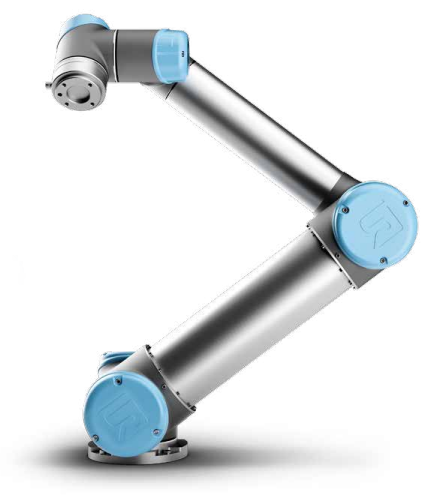
\includegraphics[width=0.5\linewidth]{img/ur5robot.png}
	\caption{UR5 kollaboratív robot}
	\label{fig:ur5}
\end{figure}


\subsection{Hivatkozások}

Ez itt egy folyóirat cikk \cite{journal-example}.

Ez itt egy konferencia cikk \cite{conference-example}.

Ez itt egy könyv \cite{book-example}.

Ez itt egy online forrás \cite{online-example}.

Ez itt egy disszertáció \cite{thesis-example}.

	
\subsection{Táblázatok}
Példaként itt látható egy táblázat \ref{tab:ur5}.

\begin{table}[H]
	\centering
	\begin{tabular}{|c|c|}
	    \hline
		Tulajdonság                      & Érték    \\ \hline
		kinyúlás {[}mm{]}                & 850      \\ \hline
		Szabadságfok                     & 6        \\ \hline
		Teherbírás {[}kg{]}               & 5        \\ \hline
		Súly {[}kg{]}                    & 18,4     \\ \hline
		Ismétlési pontosság {[}mm{]}     & $\pm0,1$    \\ \hline
		Teljesítményfelvétel {[}W{]}     & 90-325   \\ \hline
		Csuklók mozgástartománya {[}$^{\circ}${]} & $\pm360$    \\ \hline
		Max. csuklósebesség {[}$^{\circ}/sec${]}  & $\pm180$    \\ \hline
		Max. Tool sebesség {[}m/s{]}     & 1        \\ \hline
		Programozási nyelv               & URscript \\ \hline
	\end{tabular}
	\caption{Az UR5 robot főbb paraméterei}
	\label{tab:ur5}
\end{table}

Egy másik a \ref{tab:joint-limits} táblázat.

\begin{table}[H]
    \centering
    \begin{tabular}{|c|c|c|c|c|}
        \hline
    	Robotcsukló & \begin{tabular}[c]{@{}c@{}}min. poz.\\ {[}rad{]}\end{tabular} & \begin{tabular}[c]{@{}c@{}}max. poz.\\ {[}rad{]}\end{tabular} & \begin{tabular}[c]{@{}c@{}}max. sebesség\\ {[}rad/s{]}\end{tabular} & \begin{tabular}[c]{@{}c@{}}max. gyorsulás\\ \hline {[}rad/s\textasciicircum{}2{]}\end{tabular} \\ \hline
    	1 & -0.802 & 1.39 & 3.1 & 9 \\ \hline
    	2 & -2.25 & -0.873 & 3.1 & 9 \\ \hline
    	3 & 1.25 & 2.7 & 3.1 & 9 \\ \hline
    	4 & -3.49 & -1.41 & 3.1 & 9 \\ \hline
    	5 & -2.62 & -0.62 & 3.1 & 9 \\ \hline
    	6 & -3.14 & 2.09 & 3.1 & 9 \\ \hline
    \end{tabular}
    \caption{Másik példa táblázat}
    \label{tab:joint-limits}
\end{table}

	
\subsection{Képlet}

Ez itt a \ref{eq:keplet1} képlet:
\begin{align}
    \cos{\alpha-\beta} = \cos{\alpha}\cdot\sin{\beta}-\cos{\beta}\cdot\sin{\alpha}
    \label{eq:keplet1}
\end{align}	

	
\subsection{Felsorolás}

Ez egy felsorolás:
\begin{itemize}
	\item A felsorolás első eleme
	\item A felsorolás második eleme
	\item A felsorolás harmadik eleme
\end{itemize}










% ------------------------------------------------------

% JEGYZÉKEK, INNEN KI LEHET KOMMENTEZNI AMELYIK ESETLEG NEM KELL (de ha van ábra/táblázat akkor kötelező, irodalomjegyzék kötelező, rövidítések opcionális)

\clearpage
\section{IRODALOMJEGYZÉK}
\printbibliography[heading=none]

\clearpage
\renewcommand{\listfigurename}{ÁBRAJEGYZÉK}
\listoffigures

\clearpage
\renewcommand{\listtablename}{TÁBLAJEGYZÉK}
\listoftables

\clearpage
\section{RÖVIDÍTÉSEK}
% !TEX root = ./main.tex
\newcommand{\acronym}[2]{
    \item [\textbf{#1}] #2
}

\begin{itemize}[labelwidth=3cm,align=left,itemindent=3cm,itemsep=4pt]

% IDE LEHET HOZZÁADNI A RÖVIDÍTÉSEKET:

    \acronym{FTZ}{F to Z}
    \acronym{DSLR}{Digital Single-Lens Reflex camera}
    \acronym{SLR}{Single-Lens Reflex camera}
    \acronym{VR}{"Vibration Reduction"}\cite{Nikon_naming_convention}
    %\acronym{AF}{Autófókusz}
    \acronym{PC}{"Perspective Controll"}\cite{Nikon_naming_convention}
    \acronym{CPU}{Central Processing Unit}
    \acronym{AF}{"Autofocus"}\cite{Nikon_naming_convention}
    \acronym{AF-I}{"AF-Internal Motor"}\cite{Nikon_naming_convention}
    \acronym{AF-S}{"AF-Silent Wave Motor"}\cite{Nikon_naming_convention}
    \acronym{AF-P}{AF-Stepper Motor}\cite{Nikon_naming_convention}
    \acronym{AI}{"Automatic Indexing"}\cite{Nikon_naming_convention}
    \acronym{E}{"Electronic Diaphragm"}\cite{Nikon_naming_convention}
    \acronym{G}{"Gelded"}\cite{Nikon_naming_convention}
    \acronym{MILC}{"Mirrorless Interchangeable Lens Camera"}\cite{MILC_def}
    \acronym{IDE}{Integrated Development Environment}
    \acronym{USB}{Universal Serial Bus}
\end{itemize}





\end{document}
